% TO-DO:
% 1 classifying spaces *
% 2 Yoneda lemma finish
% 3 functorial semanticss
% 4 Kripke-Joyal semantics
% 5 Cohen forcing *
% 6 Sheaves and topos *
% 7 Heyting algebra revise *
% 8 fuzzy logic re-write

% 9 implementation of topology ***
% 10 model-based approach ***
% The model is only for working memory.  
% Even so, what does the model offer that syntax does not have?
% Need a simple semantic model to begin thinkinssg....

\input{../YKY-preamble.tex}

\usepackage{color}
\usepackage{mathtools}
\usepackage{hyperref}

\usepackage[backend=biber,style=numeric]{biblatex}
\bibliography{../AGI-book}
% \renewcommand*{\bibfont}{\footnotesize}

\usepackage{graphicx} % Allows including images
\usepackage{tikz-cd}
\usepackage{tikz}
\usepackage[export]{adjustbox}% http://ctan.org/pkg/adjustbox
\usepackage{verbatim} % for comments
% \usepackage{tikz-cd}  % commutative diagrams
% \newcommand{\tikzmark}[1]{\tikz[overlay,remember picture] \node (#1) {};}
% \usepackage{booktabs} % Allows the use of \toprule, \midrule and \bottomrule in tables
% \usepackage{amssymb}  % \leftrightharpoons
% \usepackage{wasysym} % frownie face
% \usepackage{newtxtext,newtxmath}	% Times New Roman font
% \usepackage{sansmath}

\numberwithin{equation}{subsection}

\newcommand{\underdash}[1]{%
	\tikz[baseline=(toUnderline.base)]{
		\node[inner sep=1pt,outer sep=10pt] (toUnderline) {#1};
		\draw[dashed] ([yshift=-0pt]toUnderline.south west) -- ([yshift=-0pt]toUnderline.south east);
	}%
}%

\DeclareSymbolFont{symbolsC}{U}{txsyc}{m}{n}
\DeclareMathSymbol{\strictif}{\mathrel}{symbolsC}{74}

\newcommand{\highlight}[1]{\colorbox{pink}{$\displaystyle #1$}}

\newcommand{\emp}[1]{{\color{violet}\textbf{#1}}}
\newcommand*\confoundFace{$\vcenter{\hbox{\includegraphics[scale=0.2]{../confounded-face.jpg}}}$}
\newcommand{\underconst}{
\includegraphics[scale=0.5]{UnderConst.png}}
\newcommand{\witness}{\scalebox{0.6}{$\blacksquare$}}
% \newcommand{\Heytingarrow}{\mathrel{-}\mathrel{\triangleright}}
\providecommand\Heytingarrow{\relbar\joinrel\mathrel{\vcenter{\hbox{\scalebox{0.75}{$\rhd$}}}}}

\begin{document}

\title{\cc{\bfseries\color{blue}{\Huge《AGI 逻辑导论》}}
{{\Huge《AGI logic tutorial》} }}
\author{YKY} % Your name
%\institute[] % Your institution as it will appear on the bottom of every slide, may be shorthand to save space
%{
%Independent researcher, Hong Kong \\ % Your institution for the title page
%\medskip
%\textit{generic.intelligence@gmail.com} % Your email address
%}
\date{\today} % Date, can be changed to a custom date

\maketitle

\section*{Summary}
\begin{itemize}
	\item 描述一种可以完整地解决 AGI 的 univeral logic
\end{itemize}

\tableofcontents
% \vspace*{0.5cm}
% 多谢 支持 \smiley

 \setcounter{section}{-1}
\section{Background}

我们想 \textbf{训练} 一个智能系统,训练 是一个 \textbf{机器学习} 的过程,也是一个 \emp{optimization} problem, 目标是将 \textbf{长期的奖励总和} 最大化:
\begin{equation}
\label{eqn:time-horizon}
\mbox{maximize: } \int_0^{\infty} R \, dt
\end{equation}
where $R(t)$ = reward at time $t$.  $\int_0^{\infty}$ 表示 计算 累积奖励的 \emp{time horizon}.  (我使用了微分的形式,实际应用通常是离散形式,但两者基本一样,不必深究)

俗语说「棋屎贪吃卒」,在开局初期吃卒,可能导致 $N$步之后被将死,这是\textbf{愚蠢}的行为。 所以 (\ref{eqn:time-horizon})式 令 系统必需顾及长远的利益,遂迫使它学习 \textbf{智慧}。

Architecturally, the AI is a \emp{dynamical system} that constantly updates its ``state'' $\vect{x}$ via: \footnote{Part of the state $\vect{x}$ contains \textbf{sensory input} and \textbf{action output} that allow the AI to interact with the external environment.}
\begin{equation}
\dot{\vect{x}} = \vect{f}(\vect{x})
\end{equation}
或者用离散形式表示:
\begin{equation}
\vect{x}_{t+1} = \vect{F}(\vect{x}_t)
\end{equation}
$\vect{F}$ 叫作 transition function.  或者更形象地表示:
\begin{equation}
\label{eqn:AGI-architecture}
\begin{tikzcd}
\vect{x} \arrow[in=160,out=20,loop,looseness=5,swap,"\vect{F}"]
\end{tikzcd}
\end{equation}
Our goal is to \textbf{learn} the function $\vect{F}$, implemented as a \emp{deep neural network}.  $\vect{F}$ 包含智能系统内的所有\textbf{知识}。 

\section{Structure of logic}

The central tenet of my theory is that the state $\vect{x}$ of the AI system is consisted of \emp{logic propositions} and that $\vect{F}$ plays the role of the \emp{logic consequence} operator $\vdash$:
\begin{equation}
\begin{tikzcd}[| /.tip = {Bar[scale=3]}]
% \begin{tikzcd}[arrow style = tikz, diagrams = {>={|[scale=2]}}]
\boxed{\mbox{propositions}}
\arrow[r, |-, "\vect{F}"]
& \boxed{\mbox{propositions}}
\end{tikzcd}
\end{equation}

So our goal now is to elucidate the structure of $\vdash$.  Currently the most elegant formulation is given by \emp{categorical logic} or \emp{topos theory}.

我发觉 我是一个擅长於 ``synthesize'' 的人,意思是我会看很多书,然后将各种 分散的 ideas 融合成一个 内部协调 的理论(当中大部分 ideas 不是我原创的)。

在接下来的篇幅,我会勾划一个 对於 AGI 来说是完整的 逻辑理论,而这理论 的中心思想 就是 Curry-Howard isomorphism....

\section{Curry-Howard correspondence}

Curry-Howard isomorphism 是一个很深刻的思想,如果不小心的话 甚至会觉得它讲了等於没讲。 

%The Curry-Howard correspondence is a deep connection between logic and computation (in the form of type theory).

简单来说: 当我们做 逻辑思考时,表面上有一种语法上 (syntax) 的形式,即 $A \Rightarrow B$:
\begin{equation}
\label{eqn:Curry-Howard}
\begin{aligned}
\boxed{\mbox{logic}} \quad \quad \underdash{$A \Longrightarrow B$} & \\
\boxed{\mbox{program}} \quad \quad \witness \; \stackrel{f}{\longmapsto} \; \witness \hspace*{10pt} &
\end{aligned}
\end{equation}
而在这 语法「底下」,还有一个 \emp{运算},它可以看成是执行 \emp{证明} (proof) 的工作,它将 $A$ 的证明 map 到 $B$ 的证明 (为了避免符号累赘,我将这些 ``proof witness'' 都记作 $\witness$,但它们每个是不同的).

一个传统的数学函数,例如 $f(x) = x + 2$ 用我们惯常的符号表示为:
\begin{equation}
\begin{aligned}
& \underdash{$f: \mathbb{R} \longrightarrow \mathbb{R}$} \\
& \hspace{2em} x \longmapsto x + 2
\end{aligned}
\end{equation}
这不是新的。 类似地,一个逻辑式子:
\begin{equation}
x \mbox{ 是偶数} \Longrightarrow x + 2 \mbox{ 是偶数}
\end{equation}
也不是新的。 但如果将「$x$是偶数」这个\textbf{命题},看成是一个\textbf{类型}或\textbf{集合},里面有个\textbf{证明} (witness),这个看法是新的: 
\begin{equation}
\begin{aligned}
& \underdash{$\boxed{x \mbox{ 是偶数}}$} \\
& \hspace*{45pt} \witness
\end{aligned}
\end{equation}
\tolerance=99999
This is called the \emp{Brouwer-Heyting-Kolmogorov (BHK) interpretation}.  由於这个想法比较 subtle,它不断被重复发现很多次,命名者可以包括: Brouwer-Heyting-Kolmogorov-Sch\"{o}nfinkel-Curry-Meredith-Kleene-Feys-G\"{o}del-L\"{a}uchli-Kreisel-Tait-Lawvere-Howard-\mbox{de Bruijn}-Scott-Martin-L\"{o}f-Girard-Reynolds-Stenlund-Constable-Coquand-Huet-Lambek ....

根据 HoTT (homotopy type theory),一个命题 可以\textbf{有}或\textbf{没有}证明; 如果有,则它的证明都是一样的,所以 经典逻辑命题 只可以取值 \textbf{真}或\textbf{假}。 我的理论推断: 模糊逻辑的取值 $\in [ 0,1 ]$ 是因为 fuzzy 命题的「证明」可以有很多个,而 fuzzy 命题的 \textbf{真值}是由 支持/反对 的证明的\textbf{比例}决定的(见 \S\ref{sec:fuzzy-logic})。 

% Curry-Howard isomorphism 讲的是 \emp{逻辑} 与 \emp{计算} 之间的同构,但在 1990s Lambek 加上了 \emp{category theory},所以现在不少人会讲 Curry-Howard-Lambek.  事实上,\textbf{逻辑-计算-范畴论} 这个「三角关系」之间的相互作用非常丰富,人们认为是未来发展的思想泉源。 

\begin{equation}
\nonumber
\mbox{John Baez (1961-)} \quad 
\vcenter{\hbox{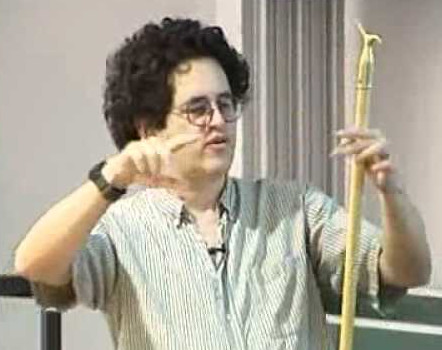
\includegraphics[scale=0.5]{Baez.jpg}}}
\end{equation}
从另一角度看,Curry-Howard isomorphism 可以看成是 某些 \emp{状态}(states,例如 $A$)和状态之间的 \emp{转换} (transitions,例如 $\stackrel{f}{\mapsto}$)之间的 \textbf{对偶}。 而这种 对偶 不断在 截然不同的范畴里出现:
\begin{equation}
\begin{tabular}{|c|c|c|c|c|}
	\hline 
	\textbf{logic} & \textbf{computation} & \textbf{category theory} & \textbf{physics} & \textbf{topology} \\ 
	\hline \hline
	proposition & type & object & system & manifold \\ 
	\hline 
	proof & term & morphism & process & cobordism \\ 
	\hline 
\end{tabular} 
\end{equation}
前两个就是 Curry-Howard,第三个 是 Lambek 加上去的,其馀的来自 John Baez \& M. Stay 的论文: \textit{Physics, Topology, Logic and Computation: a Rosetta stone} [2010].  例如在 physics 里面是 Hilbert space 和 operators 的对偶; 在 topology 里面,cobordism 的著名例子就是这个 ``pair of pants'':
\begin{equation}
\vcenter{\hbox{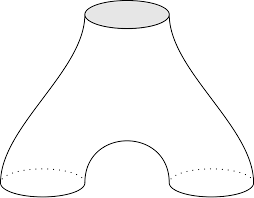
\includegraphics[scale=0.3]{pair-of-pants.png}}}
\end{equation}
In string theory,它表示上面的 strings 变成下面的 string 的「时间过程」。

\subsection{Type theory}

描述 \emp{program} 或 \emp{computation} 的语言叫 type theory.  例如在一般的 编程语言 里可以有这样的一句:
\begin{equation}
\begin{small}
\verb!define length(s: String): Integer = { .... }!
\end{small}
\end{equation}
意思是说 length() 是一个函数,输入 String,输出 Integer.

在数学里 我们描述 \emp{函数} 时会用:
\begin{equation}
f: A \rightarrow B
\end{equation}
这个表达式其实就是 type theory 的一般形式:
\begin{equation}
\overbrace{t}^{\mbox{term}} : \overbrace{T}^{\mbox{type}}
\end{equation}
而这个 notation $t:T$ 其实也可以写成 $t \in T$(但不正统而已)。 

换句话说,types 就是 \textbf{集合},terms 是集合中的 \textbf{元素}。 

更一般地,一个 type theory 的句子 可以包含 type \emp{context}:
\begin{equation}
\overbrace{x : A}^{\mbox{context}} \vdash \overbrace{f(x) : B}^{\mbox{type assignment}}
\end{equation}
意思就像在 program 的开头 ``declare'' 一些 变量 的类型,然后 program 就可以被 \emp{赋予} 后面的 类型。 

这个 $\vdash$ 的过程 称为 \emp{type assignment},而这就是 type theory 做的全部工作。 

\subsubsection{$\lambda$-calculus}

在一个 program 里,除了定义 类型,还需要定义 \emp{函数}。 这件工作是由 $\lambda$-calculus 负责。

$\lambda$-calculus 可以定义函数 而不需要提及它的「名字」。 例如,用数学式表达:
\begin{equation}
f(x) \triangleq x^2
\end{equation}
它的 $\lambda$-表达式就是:
\begin{equation}
f \triangleq \lambda x. \; x^2
\end{equation}
注意: 在 $\lambda$-表达式里,不需要提到 $f$ 的「名字」。

$\lambda$-calculus 是由 Alonso Church 发明,目的是研究数学上 \emp{substitution} 的性质。 Substitute 是每个中学生都懂得做的事,但要用数学表达出来却是出奇地麻烦。 

同时,Church 发现 $\lambda$-calculus 是一种「万有」的计算形式,和 \emp{Turing machines} 等效。 「AI 之父」John McCarthy 用 $\lambda$-calculus 发展出 \emp{Lisp} 语言,它是所有 functional programming language 的鼻祖。 

\subsubsection{Curry-Howard correspondence}

在 Curry-Howard 对应下,type $A$ 就是 逻辑命题 $A$,type $A$ 或 集合 $A$ 里面的 元素 是其 \textbf{证明} (proof, or proof witness)。

而,$A \Rightarrow B$ 也是 逻辑命题,它对应於 the function type $A \rightarrow B$,也可以写作 $B^A$,而这个 type 或 集合 里面的 元素 就是一些 函数 $f: A \rightarrow B$.  如果 有一个这样的函数存在,则 type $A \rightarrow B$ 有「住客」(inhabited),换句话说 $A \Rightarrow B$ 有 \textbf{证明}。 

\subsection{Intuitionistic logic}

Curry-Howard isomorphism 揭示了 type theory 和 \emp{intuitionistic logic} (直觉主义逻辑)之间的关系。 这种逻辑的特点是没有 \emp{排中律} (law of excluded middle, LEM),或者等价地,\emp{double negation},即 $\neg \neg p \Rightarrow p$.

排中律 是说: $p \vee \neg p$ 是 恒真命题。 但在 直觉主义 逻辑中,$p \vee \neg p$ 表示 $p$ 的证明 \textbf{或} $\neg p$ 的证明,但有时候这两者都不知道(例如 现时仍未找到证明,或者不可能找到证明)。 

附带一提: 人们惊讶地发现,在直觉主义逻辑下,axiom of choice $\Rightarrow$ law of excluded middle.  换句话说,axiom of choice 和 直觉主义 也有内在的矛盾。 

\subsubsection{Topological interpretation}

在 拓樸学 里,一般用 \emp{open sets} 表示空间中的子集(这习惯起源自 Hausdorff 时期)。  但 $p$ 的 \emp{补集} $\overline{p}$ 并不 open,所以要将 $\neg p$ 定义为 $p$ 的补集的 \emp{interior},即 $\neg p \triangleq \overline{p}^{\, \circ}$.  於是 $p \cup \neg p \neq \mbox{Universe}$: \footnote{diagram from the book: \textit{Classical and Non-classical Logics -- an introduction to the mathematics of propositions} [Eric Schechter 2005], p.126.}
\begin{equation}
\vcenter{\hbox{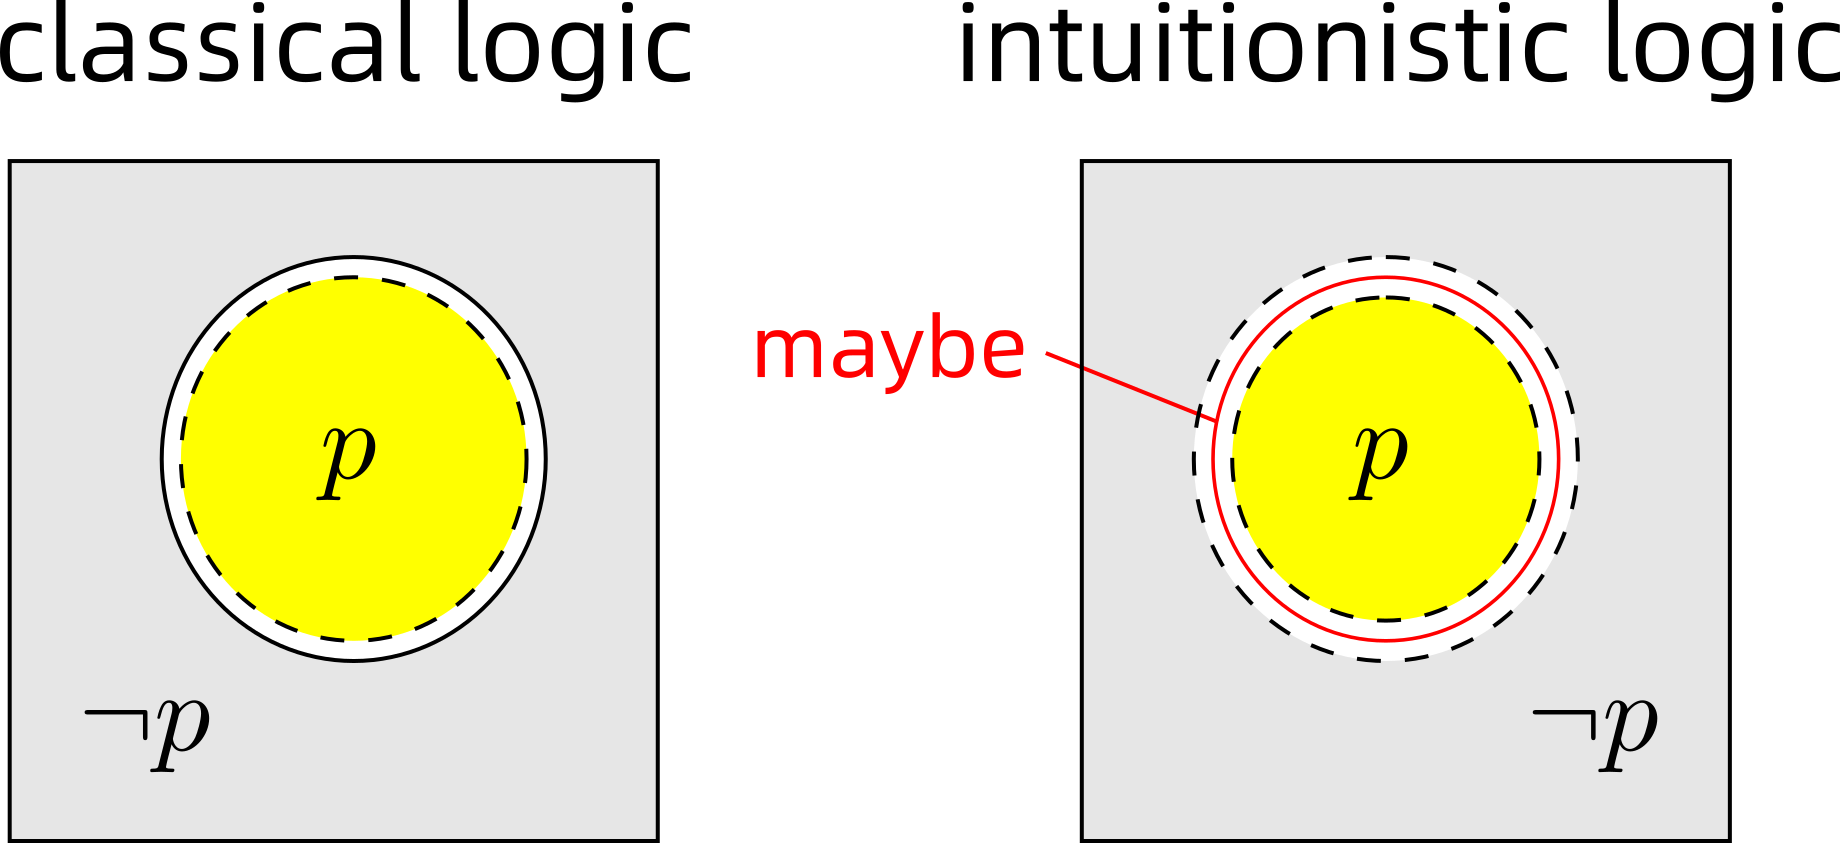
\includegraphics[scale=0.8]{topology-intuitionistic.png}}}
\end{equation}

\subsection{Higher-order logic}

Propositional logic 的意思是: 只有命题,但忽略任何 \textbf{命题内部} 的结构。 

假设 $p, q$ 是命题,命题逻辑的基本运算 就是 $p \wedge q, p \vee q, p \Rightarrow q, \neg p$.

First-order logic 的意思是: 容许 这样的方法 构成 命题:
\begin{equation}
\overbrace{\mbox{IsHuman}}^{\mbox{predicate}} ( \overbrace{\mbox{John}}^{\mbox{object}} ).
\end{equation}
Predicate 的意思是 \emp{谓词}; 谓词 是一些「有洞的命题」,它们被填入 objects 之后就变成完整的命题。 类似地可以有 \emp{多元}的 predicates,例如:
\begin{equation}
\mbox{Loves} (\mbox{John}, \mbox{Mary}).
\end{equation}
First-order 指的是: $\forall, \exists$ 这些 \emp{量词} 可以 \textbf{作用} 在 objects 的类别上,例如(Mary \textit{人见人爱}):
\begin{equation}
\forall x. \; \mbox{Loves}(x, \mbox{Mary})
\end{equation}
但 first-order logic 不容许 量词 作用在 predicates 的类别上,除非用 second-order logic.

一个 二阶逻辑的例子是「\textit{拿破仑 具有一个好将军应该具备的所有特质}」:
\begin{equation}
\forall p. \; p(\mbox{Good General}) \Rightarrow p(\mbox{Napoleon}).
\end{equation}
注意 $p$ 是在 predicates 的类别之上量化的。

\subsection{旧式 logic with type theory}

Type theory 的历史还可以追溯更早。 它起源於 Russell 为了解决 \emp{逻辑悖论},例如:「\textit{一个只帮自己不理发的人理发的理发师帮不帮自己理发?}」  这些 逻辑悖论 根源是在於: 定义一样东西的时候,中途 \textbf{指涉} 了这个东西本身。 这种不良的定义称作 \emp{impredicative}.  为了避免不良定义,每个东西出现之前必需「宣告」它的类型,这就是 type theory 原来的目的。 

在 Curry-Howard isomorphism 未被重视之前,有一种更简单地 用 type theory 定义 逻辑的方法。 在这种方法下,逻辑命题 $p, q, p \wedge q$ 等 \textbf{直接用} terms 定义,而不是像 Curry-Howard 那样,逻辑命题 = types,证明 = terms.

在这情况下 type theory 处理的是 (first- or higher-order) predicate logic 的方面。 这是说,例如:
\begin{equation}
\mbox{IsHuman} (\mbox{John})
\end{equation}
里面 IsHuman 是一个 函数 term,它输入一个 物体,输出它是不是「人」的真值 (truth value) $\in \Omega = \{ \top, \bot \}$.  因此 IsHuman 是一个 类型为 $\mbox{Obj} \rightarrow \Omega$ 的 term.

\cc{
这种做法没有容纳 Curry-Howard isomorphism 的馀地。 如果要做到后者,需要的是 Martin-L\"{o}f type theory....}{
This approach leaves no room to accommodate Curry-Howard isomorphism.  To do the latter, we would need Martin-L\"{o}f type theory....
}

\subsection{Martin-L\"{o}f type theory}
\label{sec:Martin-Lof-TT}

根据 Curry-Howard, 下面的 $A {\color{blue}\Rightarrow} B$ 是一个 逻辑命题,因而是一个 type: 
\begin{equation}
\label{eqn:2-levels-of-TT}
\vcenter{\hbox{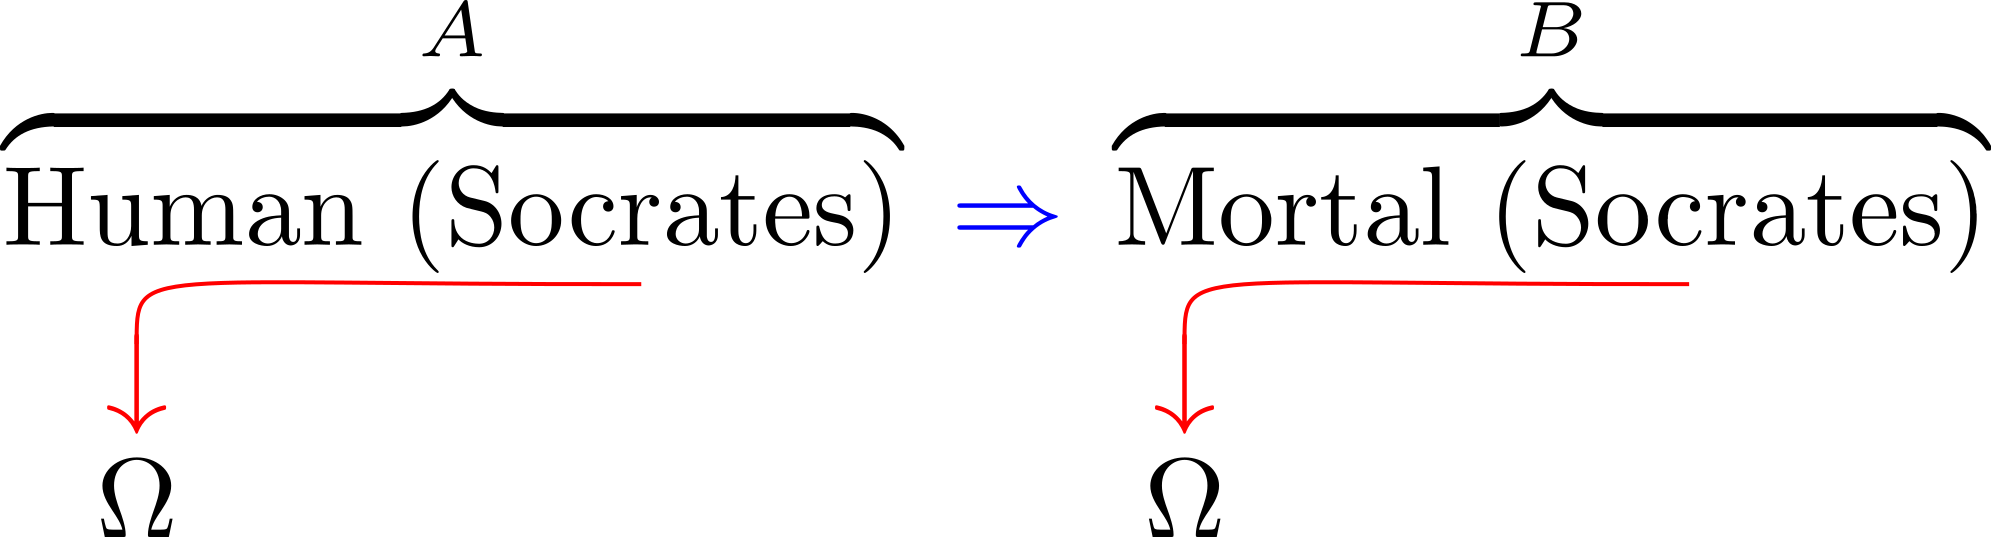
\includegraphics[scale=0.8]{why-Martin-Lof.png}}}
\end{equation}
但另方面,Human() 和 Mortal() 这两个 predicates 也需要借助 type theory 来构成命题,它们也是 types.  ${\color{red}\mbox{红色} \rightarrow}$ 和 ${\color{blue}\mbox{蓝色} \Rightarrow}$ 的两个层次 是完全不同的 两码子事,但因为 Curry-Howard 而被逼 挤在一起。 这就使得 type theory 好像「一心不能二用」。

在 ``simple'' type theory 里面可以 构造:
\begin{itemize}
	\item sum type $A + B$
	\item product type $A \times B$
	\item function type $A \rightarrow B$
\end{itemize}
分别对应於 直觉主义逻辑的 $\vee, \wedge, {\color{blue}\Rightarrow}$.  这些是在 \textbf{命题逻辑} 层面的,已经「用尽」了 type theory 的法宝。 

但 Human(Socrates) 也是由 Human() 和 Socrates 构成的命题,这构成的方法是用一个 arrow ${\color{red}\rightarrow}$,但已经没有 arrow 可用。 

Martin-L\"{o}f 提出的解决方案是 引入新的 \emp{type constructors}:
\begin{itemize}
	\item \textbf{dependent} sum type $\Sigma$
	\item \textbf{dependent} product type $\Pi$
\end{itemize}

Dependent sum $\displaystyle \sum_A B$ 里面 $B$ 的类型 depends on $A$. 整个 family of A 的 + 的结果变成类似 product $A \times B$.

Dependent product $\displaystyle \prod_A B$ 里面 $B$ 的类型 depends on $A$. 整个 family of A 的 $\times$ 的结果变成类似 exponentiation $B^A$.

Dependent products can be used to define \textbf{predicates} such as Human() and Mortal().  They are of type $\displaystyle \mathrm{Obj} \rightarrow \Omega = \Omega^{\mathrm{Obj}} = \prod_{\mathrm{Obj}} \Omega$.  \footnote{Note that ``objects'' here mean logic objects, not objects in category theory.}

一个很漂亮的结果是: 如果用 $\sum_A B$ 和 $\prod_A B$ 定义 逻辑命题,则这些 types 如果被 inhabited 的话,分别对应於 $\exists A. B(A)$ 和 $\forall A. B(A)$. 这是因为: 如果 $A \times B$ inhabited,表示\textbf{至少存在}一个 $B(A)$; 而如果 $B^A$ inhabited,则存在一个函数,将\textbf{任意的} $A$ send to $B$.

Per Martin-L\"{o}f (1942-) was the first logician to see the full importance of the connection between intuitionistic logic and type theory.
\begin{equation}
\nonumber
\mbox{Per Martin-L\"{o}f (1942-)} \quad \vcenter{\hbox{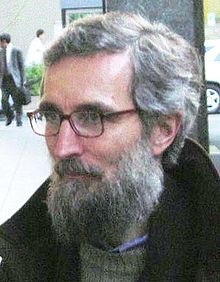
\includegraphics[scale=0.5]{Martin-Lof.jpg}}}
\end{equation}

\subsection{Arithmetic-logic correspondence}

很多人都知道,经典逻辑中 $\wedge, \vee$ 对应於 \textbf{算术运算} $\times, +$(也可以看成是 fuzzy logic 的 $\min, \max$.) 其实这就是 George Boole 尝试将 \emp{逻辑} 变成 某种\emp{代数} 的原因。

较少人知道的是 $A \Rightarrow B$ 也对应於 $B^A$: \footnote{其中 $0^0$ 是「不确定式」,但按照 组合学 惯例可以定义为 1.}
\begin{equation}
\label{truth-table:material-implication}
\begin{tabular}{|c|c|c|c|}
	\hline 
	$A$ & $B$ & $A \Rightarrow B$ & $B^A$ \\ 
	\hline \hline 
	0 & 0 & 1 & $0^0 = 1$ \\
	\hline 
	0 & 1 & 1 & $1^0 = 1$ \\ 
	\hline 
	1 & 0 & 0 & $0^1 = 0$ \\ 
	\hline 
	1 & 1 & 1 & $1^1 = 1$ \\ 
	\hline 
\end{tabular} 
\end{equation}
这个惊奇的「巧合」似乎再一次证实 Curry-Howard correspondence 是正确的; 特别地,它意味 $\Rightarrow$ 应该看成是 \textbf{函数},即所谓 ``functional interpretation of logical deduction.'' 

\subsection{The problem of material implication}
\label{sec:material-implication}

更详细观察,table (\ref{truth-table:material-implication}) 里面 $A$ 和 $B$ 的 truth values 可以看成是它们的 types 有没有 \textbf{inhabitants}. Type $A$ 的 inhabitant 就是它的证明 $\witness$,没有证明就是 $\emptyset$.  或者推广到:命题 $A$ 的真值 = $A$ 的 type 作为 集合 的 \textbf{cardinality}; The truth valuation of $A = |A|$.  这样看,$A \Rightarrow B$ 的真值 就是 $|B^A|$, 亦即是从 $\{\witness\}$ 或 $\emptyset$ 到 $\{\witness\}$ 或 $\emptyset$ 的 map 的个数, 而这个 map 只有在 $\emptyset \mapsto \{\witness\}$ 的时候是空集(不可能)。

这个观察 可以推广到 fuzzy logic (\S\ref{sec:fuzzy-implication}) 和 strict implication $A \strictif B$ (\S\ref{sec:strict-implication}).

但 material implication 导致某种悖论:
\begin{equation}
A \wedge B \quad \vdash \quad A \Rightarrow B
\end{equation}
例如
\begin{equation}
\mbox{看见黑猫} \wedge \mbox{发生车祸} \quad \vdash \quad \mbox{看见黑猫} \Rightarrow \mbox{发生车祸}
\end{equation}
即任何两件\textbf{同时}发生的事件,会导致类似\textbf{因果}的结论,然而这因果关系未必成立。 这个谬误出现的原因,似乎是因为混淆了不同时间的 \emp{cases}.  换句话说: 我们应该验证了 table (\ref{truth-table:material-implication}) 的所有 cases,然后才下结论说 $A \Rightarrow B$; 然而根据 经典逻辑的 material implication,只需要一个 case 就可以下结论说 $A \Rightarrow B$.

那么,这个谬误 为什么没有在 经典逻辑 AI 系统中被发现?

所谓 \emp{inductive learning of logic rules},其原理是根据以下的「生成模型」: 
\begin{equation}
\begin{tikzcd}[| /.tip = {Bar[scale=3]}, column sep = large]
\mbox{generators} \arrow[|-,r, "\mathrm{generate}"]
& \mbox{data of the world}
\end{tikzcd}
\end{equation}
这种 generators 的思想,和 数学中 generators of ideals, groups, function fields, 等 是一样的。 

Machine learning 的目的,是求得一组这样的 generators,而它生成的\textbf{机制},即是逻辑推导 $\vdash$.

但由於在 learning 的过程中,需要验证 \textbf{不同时间}的 cases,因此避免了 太轻易接受 $A \Rightarrow B$ 的问题。 

\section{Topos theory}

\section{Basics}

\begin{equation}
\nonumber
\mbox{Joachim Lambek (1922-2014)} \quad \vcenter{\hbox{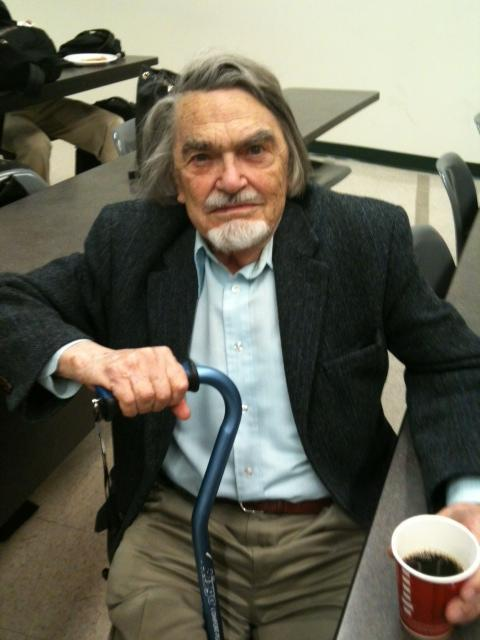
\includegraphics[scale=0.4]{Lambek.jpg}}}
\end{equation}
将 type theory 对应到 category theory,这工作是 Lambek 做的,於是完成了 Curry-Howard-Lambek 的「三位一体」:
% \tikzcdset{arrows={line width=3pt}}
\begin{equation}
\begin{tikzcd}[column sep = -1em]
\mbox{logic} \arrow[-,rr,line width=1.5pt] \arrow[-,dr]
&& \mbox{programming} \arrow[-,dl] \\
& \mbox{category theory}
\end{tikzcd}
\end{equation}

Topos 的重要意义在於 它是一个可以用来 \textbf{进行逻辑运算} 的范畴,关键在於它可以表达 \textbf{子集} 的概念,或更一般地叫作 \emp{sub-objects}.

一个 topos $\mathcal{C}$ 里面存在 sub-object classifer $\Omega$ 使得 $X \rightarrow \Omega \cong \mbox{sub-objects of } X$.  换句话说 $X$ 的 子集 可以用 $X \rightarrow \Omega$ 这个映射来 \emp{represent}.

在 $\mathbf{Set}$ 这个 topos 里面,$\Omega$ 是一个有\textbf{两个}元素的集合,可以记作 $\{ \top, \bot \}$.  那么 $X \rightarrow \Omega$ 就是一些 \emp{命题},例如 $X$ 是人的集合,则 $\begin{tikzcd}[column sep = 12ex]
X \arrow[r, "\mathrm{mathematician}"] & \Omega \end{tikzcd}$ 定义哪些人是数学家。 

Topos theory 里面最重要的 commutative diagram 是这个:
\begin{equation}
\label{eqn:subobject-classifier}
\begin{tikzcd}[column sep = normal]
X \arrow[r, "!"] \arrow[d, tail, swap, "m"] & 1 \arrow[d, "\mathrm{true}"] \\
Y \arrow[r, swap, "\Chi_m"] & \Omega
\end{tikzcd}
\end{equation}
其中:
\begin{itemize}
	\item $X \stackrel{!}{\longrightarrow} 1$ 是个 unique arrow,它将 集合 $X$ \textbf{整个地}映射到 1. 而 1 是 terminal object,它的定义就是说,通向它的箭咀只能有一个。

	\item $\begin{tikzcd}1 \arrow[r, "\mathrm{true}"] & \Omega \end{tikzcd}$ 在 $\top$ 和 $\bot$ 之间选择 $\top$, 因此叫 ``true'' arrow.

	\item $\begin{tikzcd}X \arrow[r, tail, "m"] & Y \end{tikzcd}$ 是 \emp{monic} arrow,特别地,在 $\mathbf{Set}$ 里面它就是 \emp{inclusion} map,即 $\begin{tikzcd}X \arrow[r, hook, "m"] & Y \end{tikzcd}$.  它表示 $X$ 是 $Y$ 的\textbf{子集},$X \subseteq Y$.

	\item $\begin{tikzcd}Y \arrow[r, "\Chi_m"] & \Omega \end{tikzcd}$ 是集合论中熟悉的 \emp{characteristic function}, 当元素 $e \in X \subseteq Y$ 时,$\Chi(e)$ 取值 1,否则为 0.  正是 $\Chi_m$ 的存在令这幅图 commute.  $\Chi_m$ 也记作 $\ulcorner m \urcorner$.
\end{itemize}
不熟悉基本范畴论的读者,我非常推荐看一看《Conceptual Mathematics》这本书,写得连中学生也可以看懂,而作者之一的 Lawvere 正是 topos 理论的创始人。 

从 $\mathbf{Set}$ 的角度看,这个 diagram 很易理解,但 topos 的好处是它可以将这些逻辑概念 \textbf{generalize} 到比 $\mathbf{Set}$ 更一般的范畴。 

Topos 理论的重要性 在於 它用 category 的语言 \textbf{重新表述}了 集合论的整个基础。 特别地,逻辑学中的符号,例如 $P(x), \forall x, \exists x,$ 表面上看似无法用范畴论表示,这正是 Lawvere 惊人的成就。 
\begin{equation}
\nonumber
\mbox{William Lawvere (1937-)} \quad 
\vcenter{\hbox{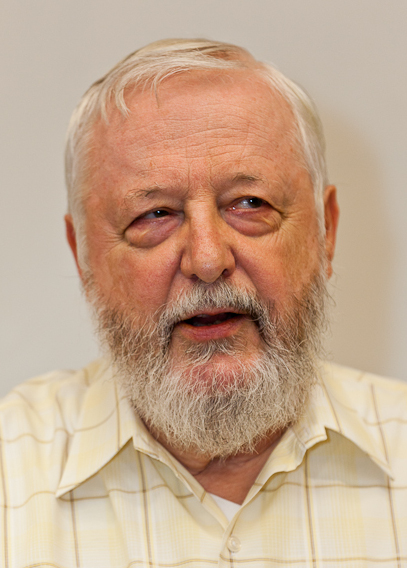
\includegraphics[scale=1.0]{Lawvere.jpg}}}
\end{equation}

再看一次 图 (\ref{eqn:subobject-classifier}):
\begin{equation}
\begin{tikzcd}[column sep = normal]
X \arrow[r, "!"] \arrow[d, tail, swap, "m"] \arrow[dr, phantom, "\lrcorner", red, very near start] & {\color{red}1} \arrow[d, red, "\mathrm{true}"] \\
Y \arrow[r, swap, "\ulcorner m \urcorner"] & {\color{red}\Omega}
\end{tikzcd}
\end{equation}
右边的 ${\color{red}\mathrel{\substack{1\\\downarrow\\\Omega}}}$ 称为 \emp{generic subobject}.  它的 \emp{pull back} square 用 ${\color{red}\lrcorner}$ 记号表示。 而左边的 $\mathrel{\substack{X\\\downarrow\\Y}}$ 则是一般的 sub-object. We say that the \textbf{property} of being a sub-object is \emp{stable under pullbacks}.

\subsection{The idea of classifying spaces}

Topos 中 $Y \rightarrow \Omega$ 这个箭头,是 \emp{classifying space} 或 \emp{moduli space} 的一个特例。  这方面我不太熟悉。

A moduli space is a space whose points can be put in a 1-to-1 correspondence with the objects we are interested in.

A moduli space is a manifold, or variety, which parametrises some class of
geometric objects.  For example:
\begin{equation}
\mathcal{M} = 
 \Big\{ \begin{tabular}{l}
 equivalence classes of objects such as \\
 Reimann surfaces, algebraic curves, etc
 \end{tabular}
 \Big\}.
\end{equation}

Every family over $B$ is the pullback of $\mathcal{C}$ via a unique map from $B$ to $\mathcal{M}$:
\begin{equation}
\label{eqn:moduli-space}
\begin{tikzcd}[column sep = normal]
\mathcal{D} \arrow[r] \arrow[d, swap, "\phi"] & \mathcal{C} \arrow[d, "1"] \\
B \arrow[r, swap, "\Chi"] & \mathcal{M}
\end{tikzcd}
\end{equation}
Classifying space for principal $G$-bundles:
\begin{equation}
\begin{tikzcd}[column sep = normal]
Y \arrow[r] \arrow[d, swap, "\gamma"] & EG \arrow[d, "\pi"] \\
Z \arrow[r, swap, "\phi"] & BG
\end{tikzcd}
\end{equation}

\subsection{$\forall$ and $\exists$ as adjunctions}

Let $\mbox{Forms}(\bar{X})$ denote the set of formulas with only the variables $\bar{X}$ free. ($\bar{X}$ may contain multiple variables.)

Then one can always trivially add an additional \textbf{dummy} variable $Y$:
\begin{equation}
\delta : \mbox{Forms}(\bar{X}) \rightarrow \mbox{Forms}(\bar{X}, Y)
\end{equation}
taking each formula $\Phi(\bar{X})$ to itself.

It turns out that $\exists$ and $\forall$ are \textbf{adjoints} to the map $\delta$:
\begin{equation}
\begin{tikzcd}[column sep = large]
\mbox{Forms}(\bar{X}) 
\arrow[r, "\delta"]
& \mbox{Forms}(\bar{X},Y) 
\arrow[l, shift right=1.2em, "\exists_Y"'] % "\bot"
\arrow[l, shift left=1em, "\forall_Y"] % "\bot"'
\end{tikzcd}
\end{equation}
or simply denoted as $\exists \dashv \delta \dashv \forall$.  \cc{而这是十分 makes sense 的,因为 一个 $\Phi(\bar{X},Y)$ 的式子,经过 $\forall Y. \; \Phi(\bar{X},Y)$ 之后,就变成一个和 $Y$ \textbf{无关}的式子。}
{This makes a lot of sense, because a formula $\Phi(\bar{X},Y)$, after being quantified as $\forall Y. \; \Phi(\bar{X},Y)$, turns into a formula that is \textbf{independent} of $Y$.}

In \textbf{cylindric algebra}, the quantifiers $\forall_Y$ and $\exists_Y$ can be interpreted as \textbf{projections} where $Y$ is the component that is ``killed'' by the projections:
\begin{equation}
\vcenter{\hbox{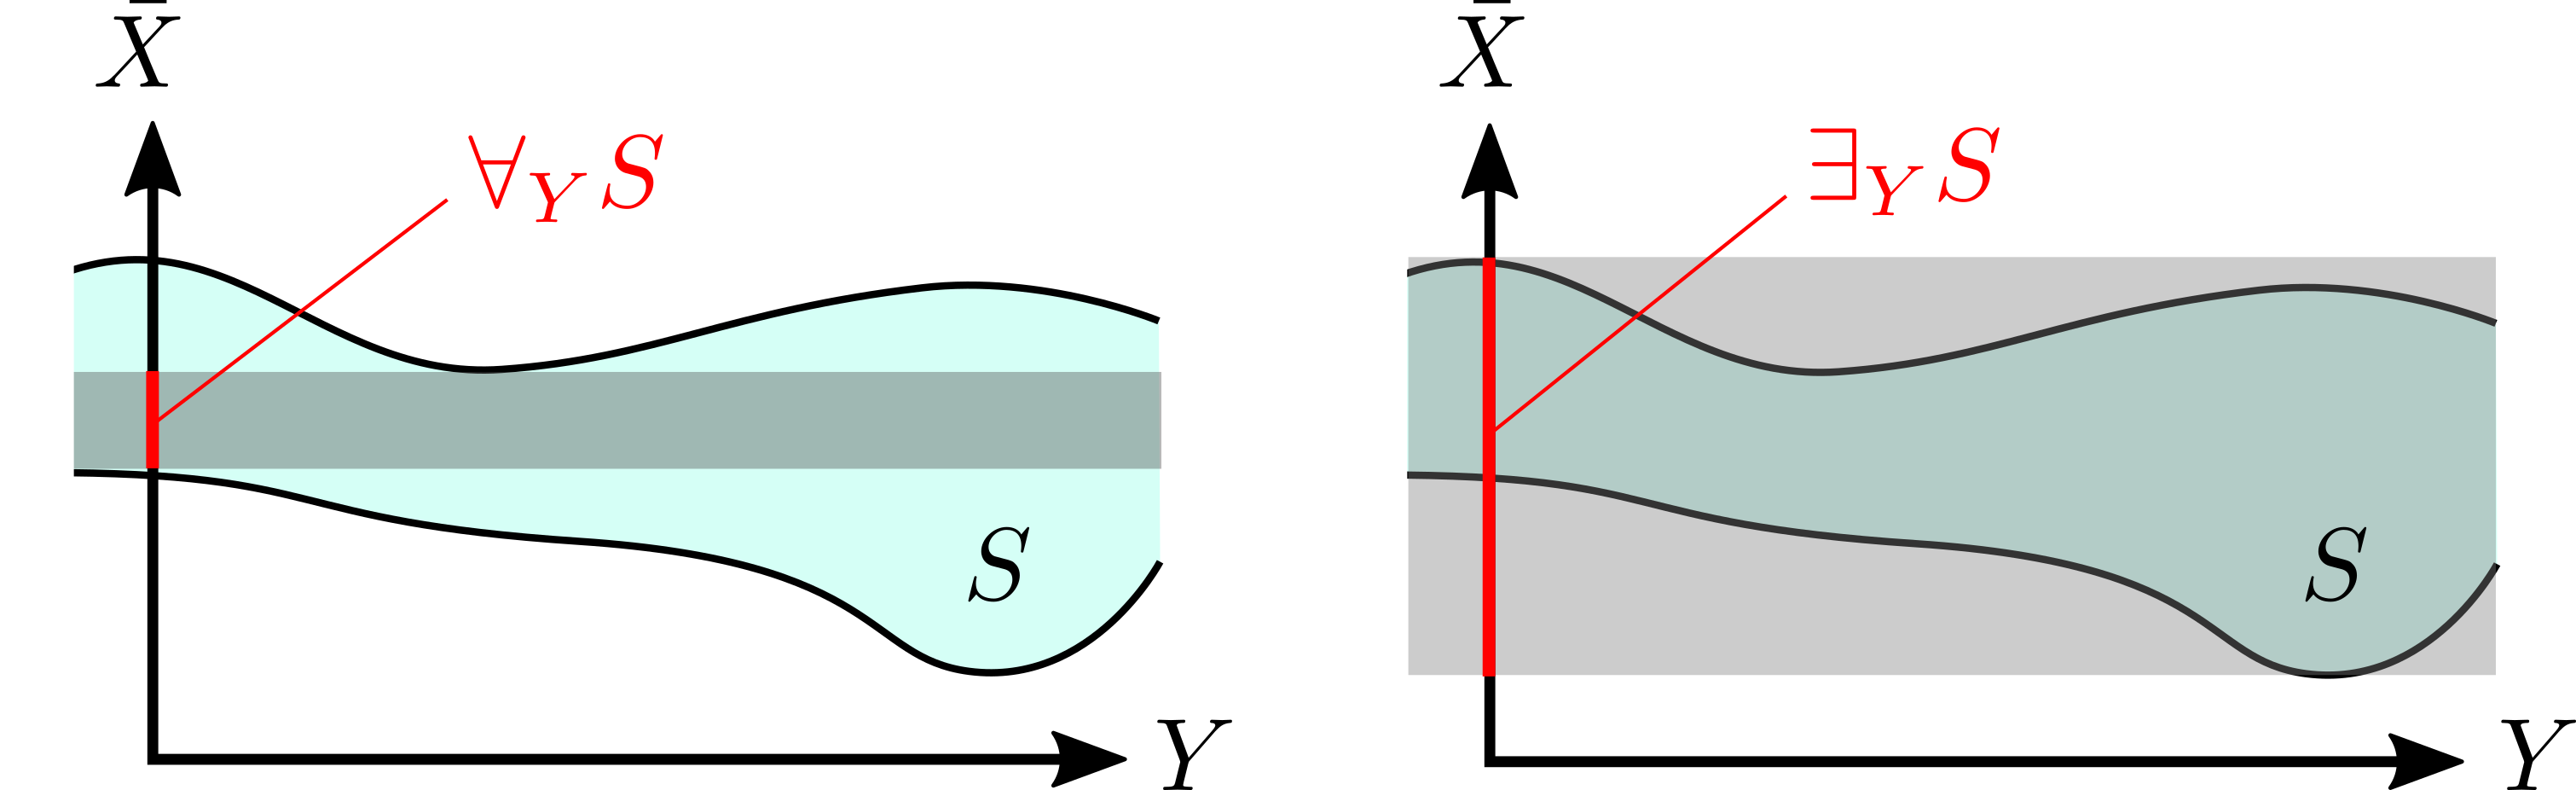
\includegraphics[scale=0.7]{cylindrification-projected.png}}}
\end{equation}

\cc{另一个方法是 借助 $T$ 定义}
{Another way is to define with the help of a variable set $T$}
\footnote{This formula is from \parencite{Abramsky2011} } (\cc{注意 在下图中 $\bar{X}$ 和 $Y$ 变成平面):}
{(Note that $\bar{X}$ and $Y$ are show as 2D domains below) :}
% \color[rgb]{0.0,0.5,0.0}  %% dark blue
\begin{eqnarray}
\label{eqn:Abramsky-1}
\forall T \subseteq \bar{X}: \qquad 
&S \subseteq \delta^{-1} (T) \qquad \Longleftrightarrow \qquad \exists {}_Y  S \subseteq T& \\
&\vcenter{\hbox{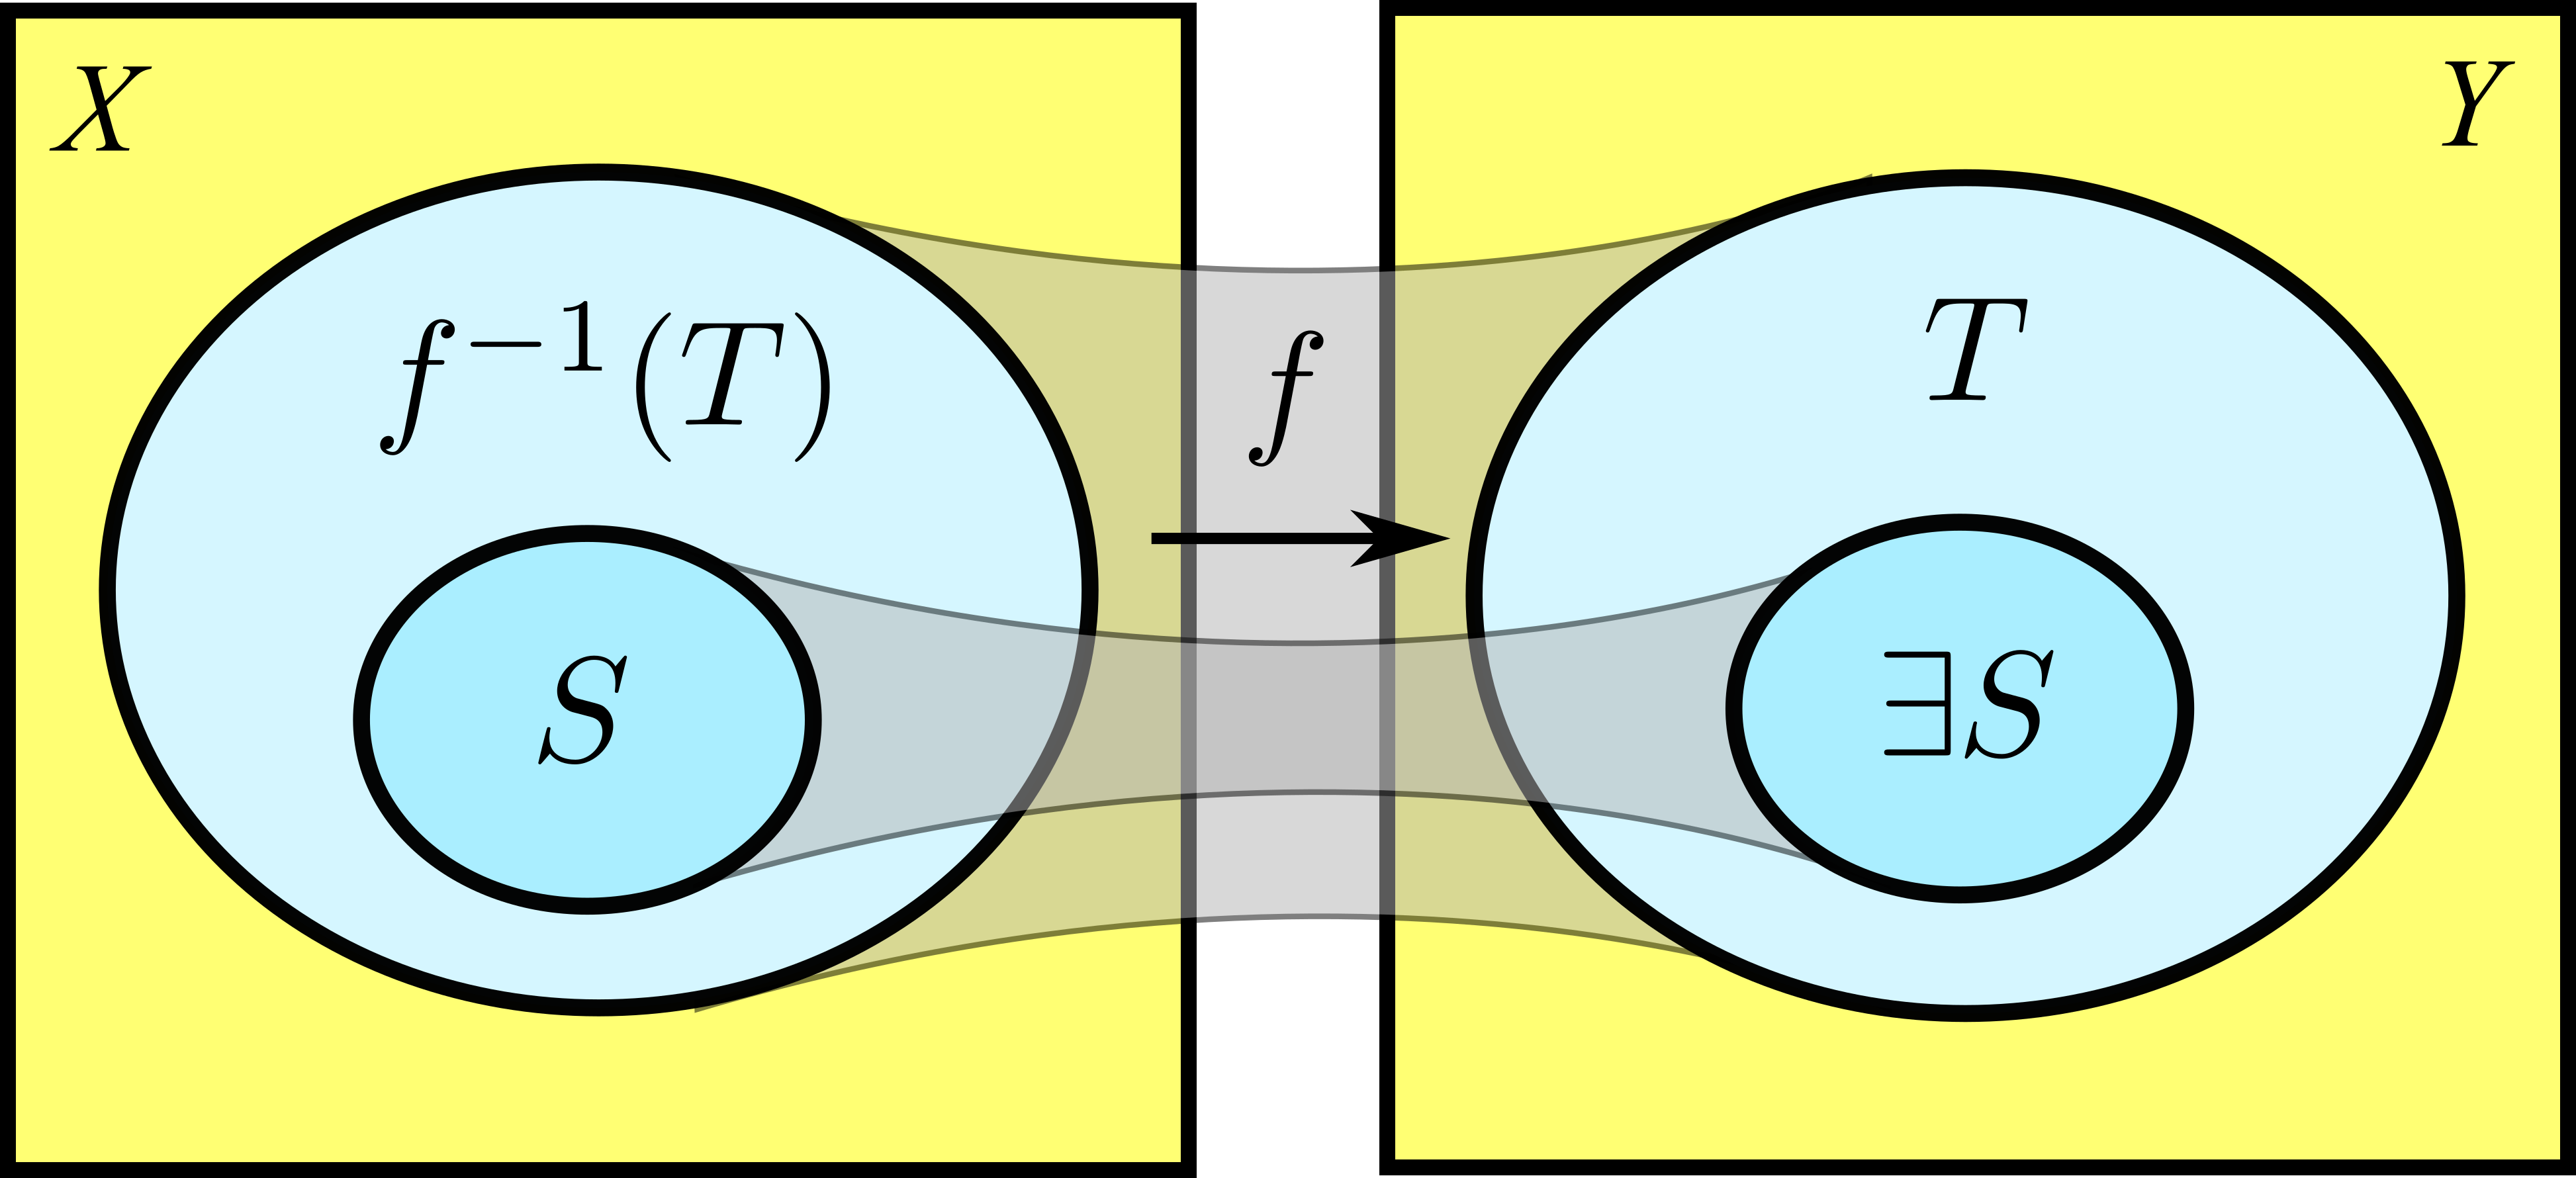
\includegraphics[scale=0.7]{Lawvere-quantifier-exists.png}}}& \nonumber
\end{eqnarray}
\cc{熟悉 Galois theory 的读者 可以理解 adjunction 是 \textbf{Galois connection} 的推广形式。 用日常语言讲: 我们知道 $S$,想定义 $\exists S$; $S$ 存在於论域 $Y$,$\exists S$ 存在於 论域 $\bar{X}$; 借助「影子」$T$ 在 论域 $\bar{X}$ 夹著 $\exists S$,则影子的「原象」在论域 $Y$ 夹著 $S$.  下图是 $\delta$ 是 projection 的特例, $\delta$ 是「杀掉」$Y$ 的 projection:}
{Readers familiar with Galois theory may understand adjunctions as a generalization of \textbf{Galois connections}.  In everyday language:  We know $S$, and would like to define $\exists S$.  $S$ lives in the domain  $Y$, $\exists S$ in the domain $\bar{X}$.  We seek the help of a ``shadow'' $T$ in domain $\bar{X}$ to get ahold of $\exists S$, and the shadow's ``original'' in domain $Y$ would be holding $S$.  The following is a special case where $\delta$ is a projection, one that ``kills'' the dimension $Y$:}
\begin{equation}
\label{fig:Lawvere-cylindrification-exists}
\vcenter{\hbox{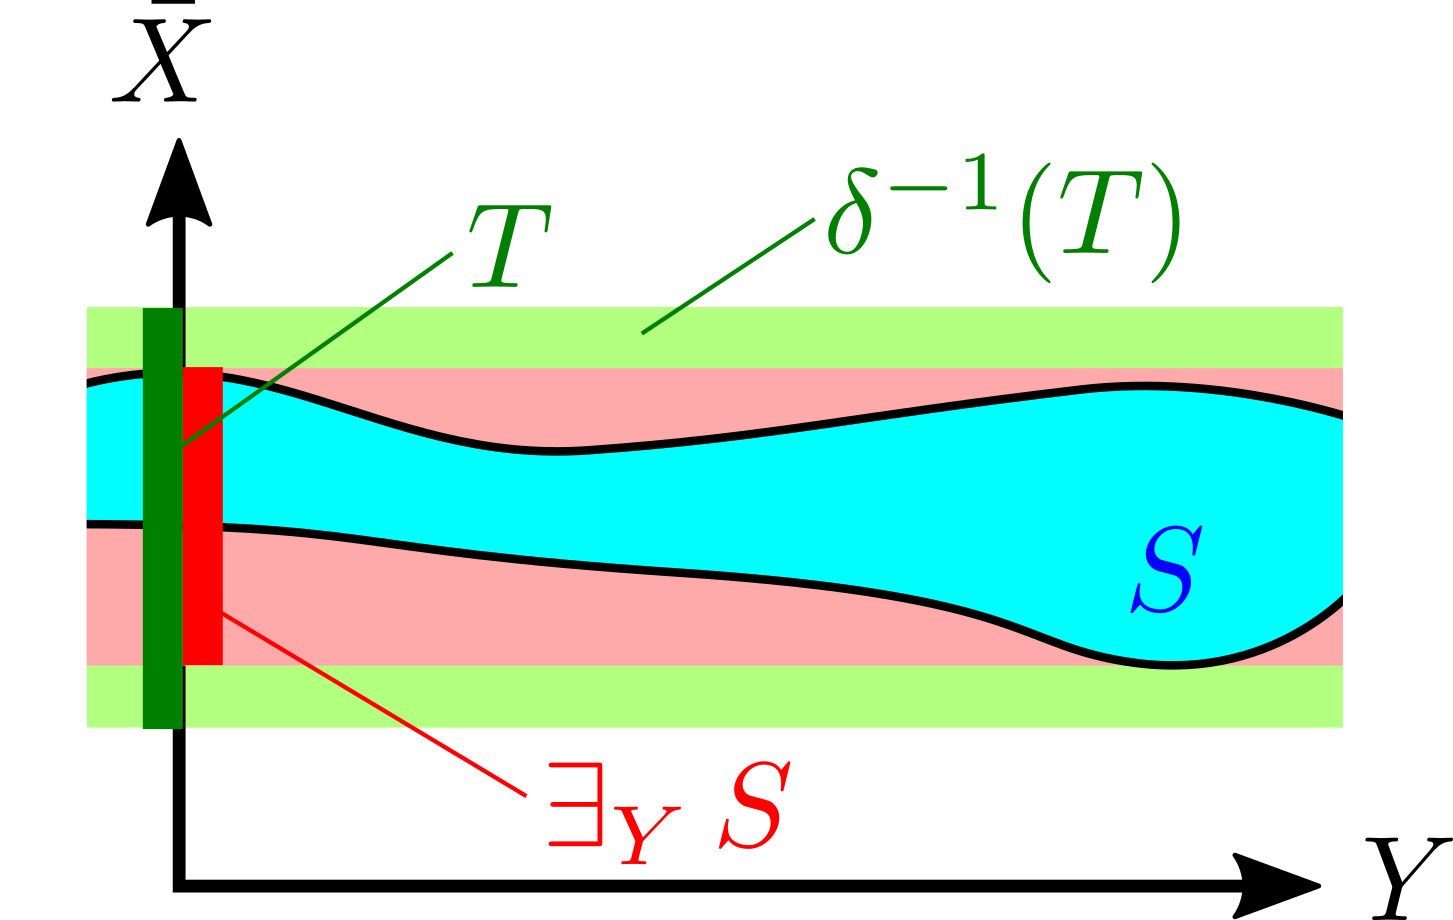
\includegraphics[scale=0.7]{Lawvere-cylindrification-exists.png}}}
\end{equation}
\cc{注意: (\ref{fig:Lawvere-cylindrification-exists}) 的 $\delta$ 是 $\bar{X} \times Y \rightarrow X$ 的 projection,但 (\ref{eqn:Abramsky-1}) 的 $\delta$ 可以是\textbf{任何} $Y \rightarrow X$ 的映射,这似乎是 $\forall$ 和 $\exists$ 的最一般的定义。 范畴论 定义 的好处是 方便推广到其他逻辑「模型」,例如 过渡到 Banach space.}
{Note that in (\ref{fig:Lawvere-cylindrification-exists}), $\delta$ is a projection from $\bar{X} \times Y \rightarrow X$, but the $\delta$ in (\ref{eqn:Abramsky-1}) can be \textbf{any} map $Y \rightarrow X$, and this seems to be the most general definition of $\forall$ and $\exists$.  The advantage of using categorical definitions is that they can be easily transferred to other categories, such as Hilbert space.}

\cc{类似地有 $\forall$ 的定义:}
{Similarly we have the definition of $\forall$:}
\begin{eqnarray}
\forall T \subseteq \bar{X}: \qquad 
&\delta^{-1} (T) \subseteq S \qquad \Longleftrightarrow \qquad T \subseteq \forall {}_Y S& \\
&\vcenter{\hbox{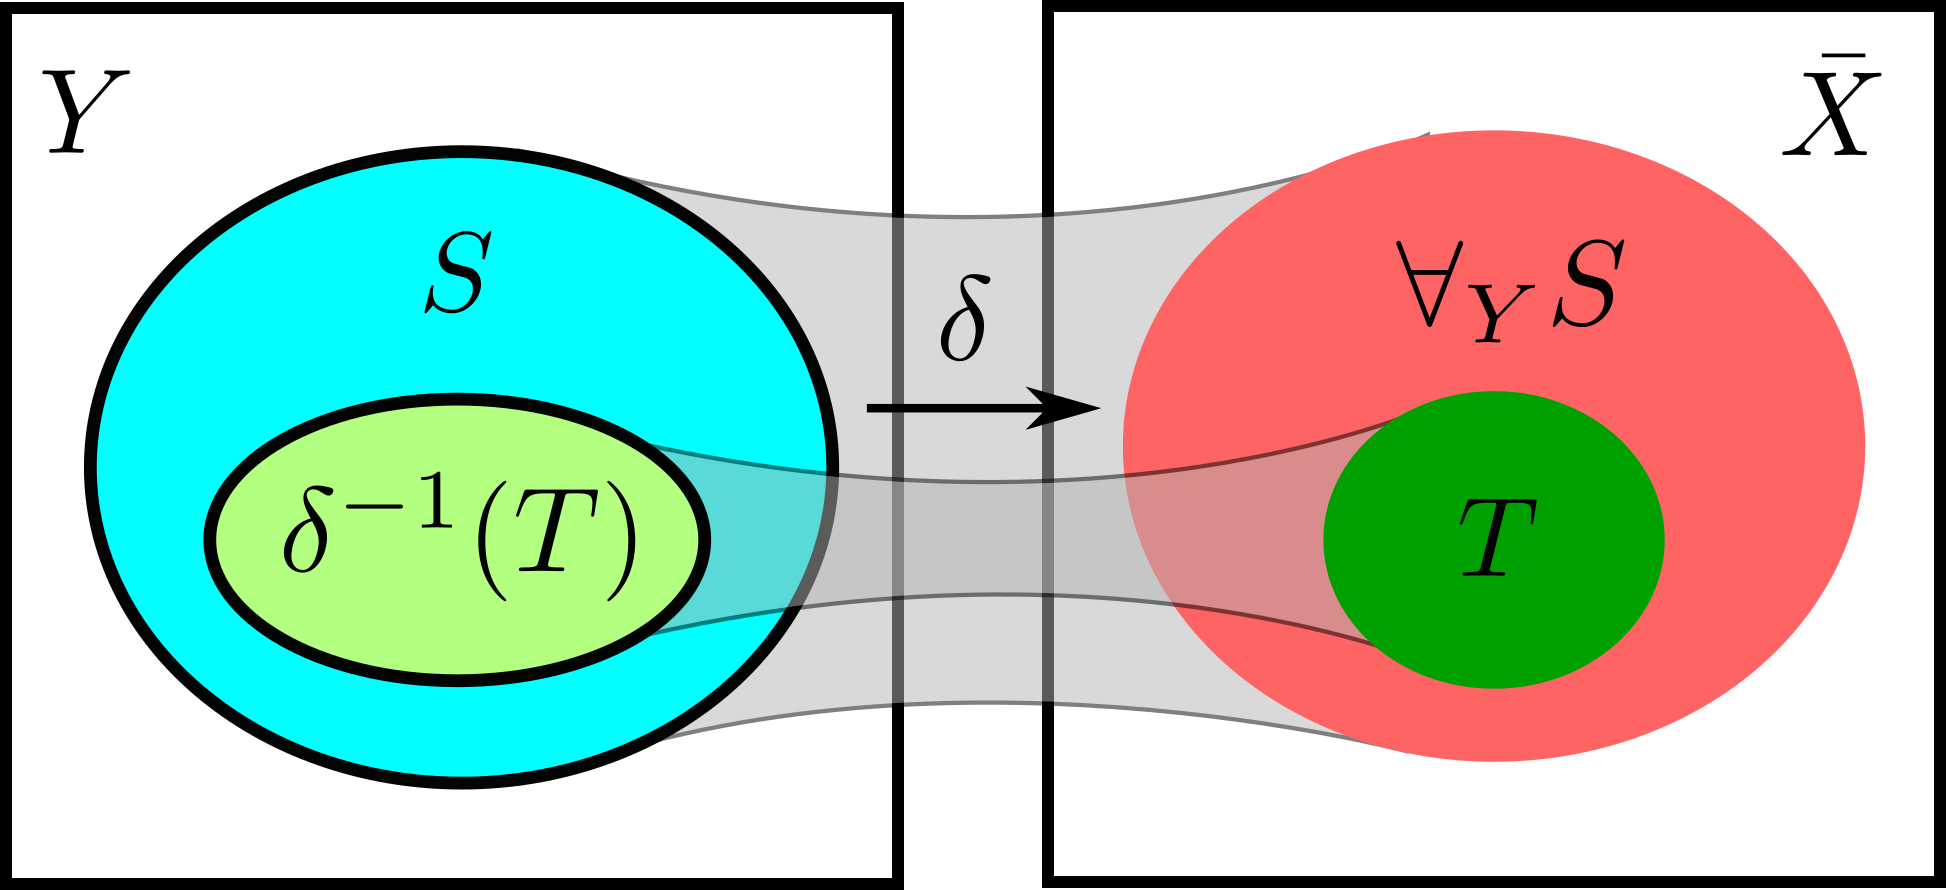
\includegraphics[scale=0.7]{Lawvere-quantifier-forall.png}}}& \nonumber
\end{eqnarray}
\begin{equation}
\vcenter{\hbox{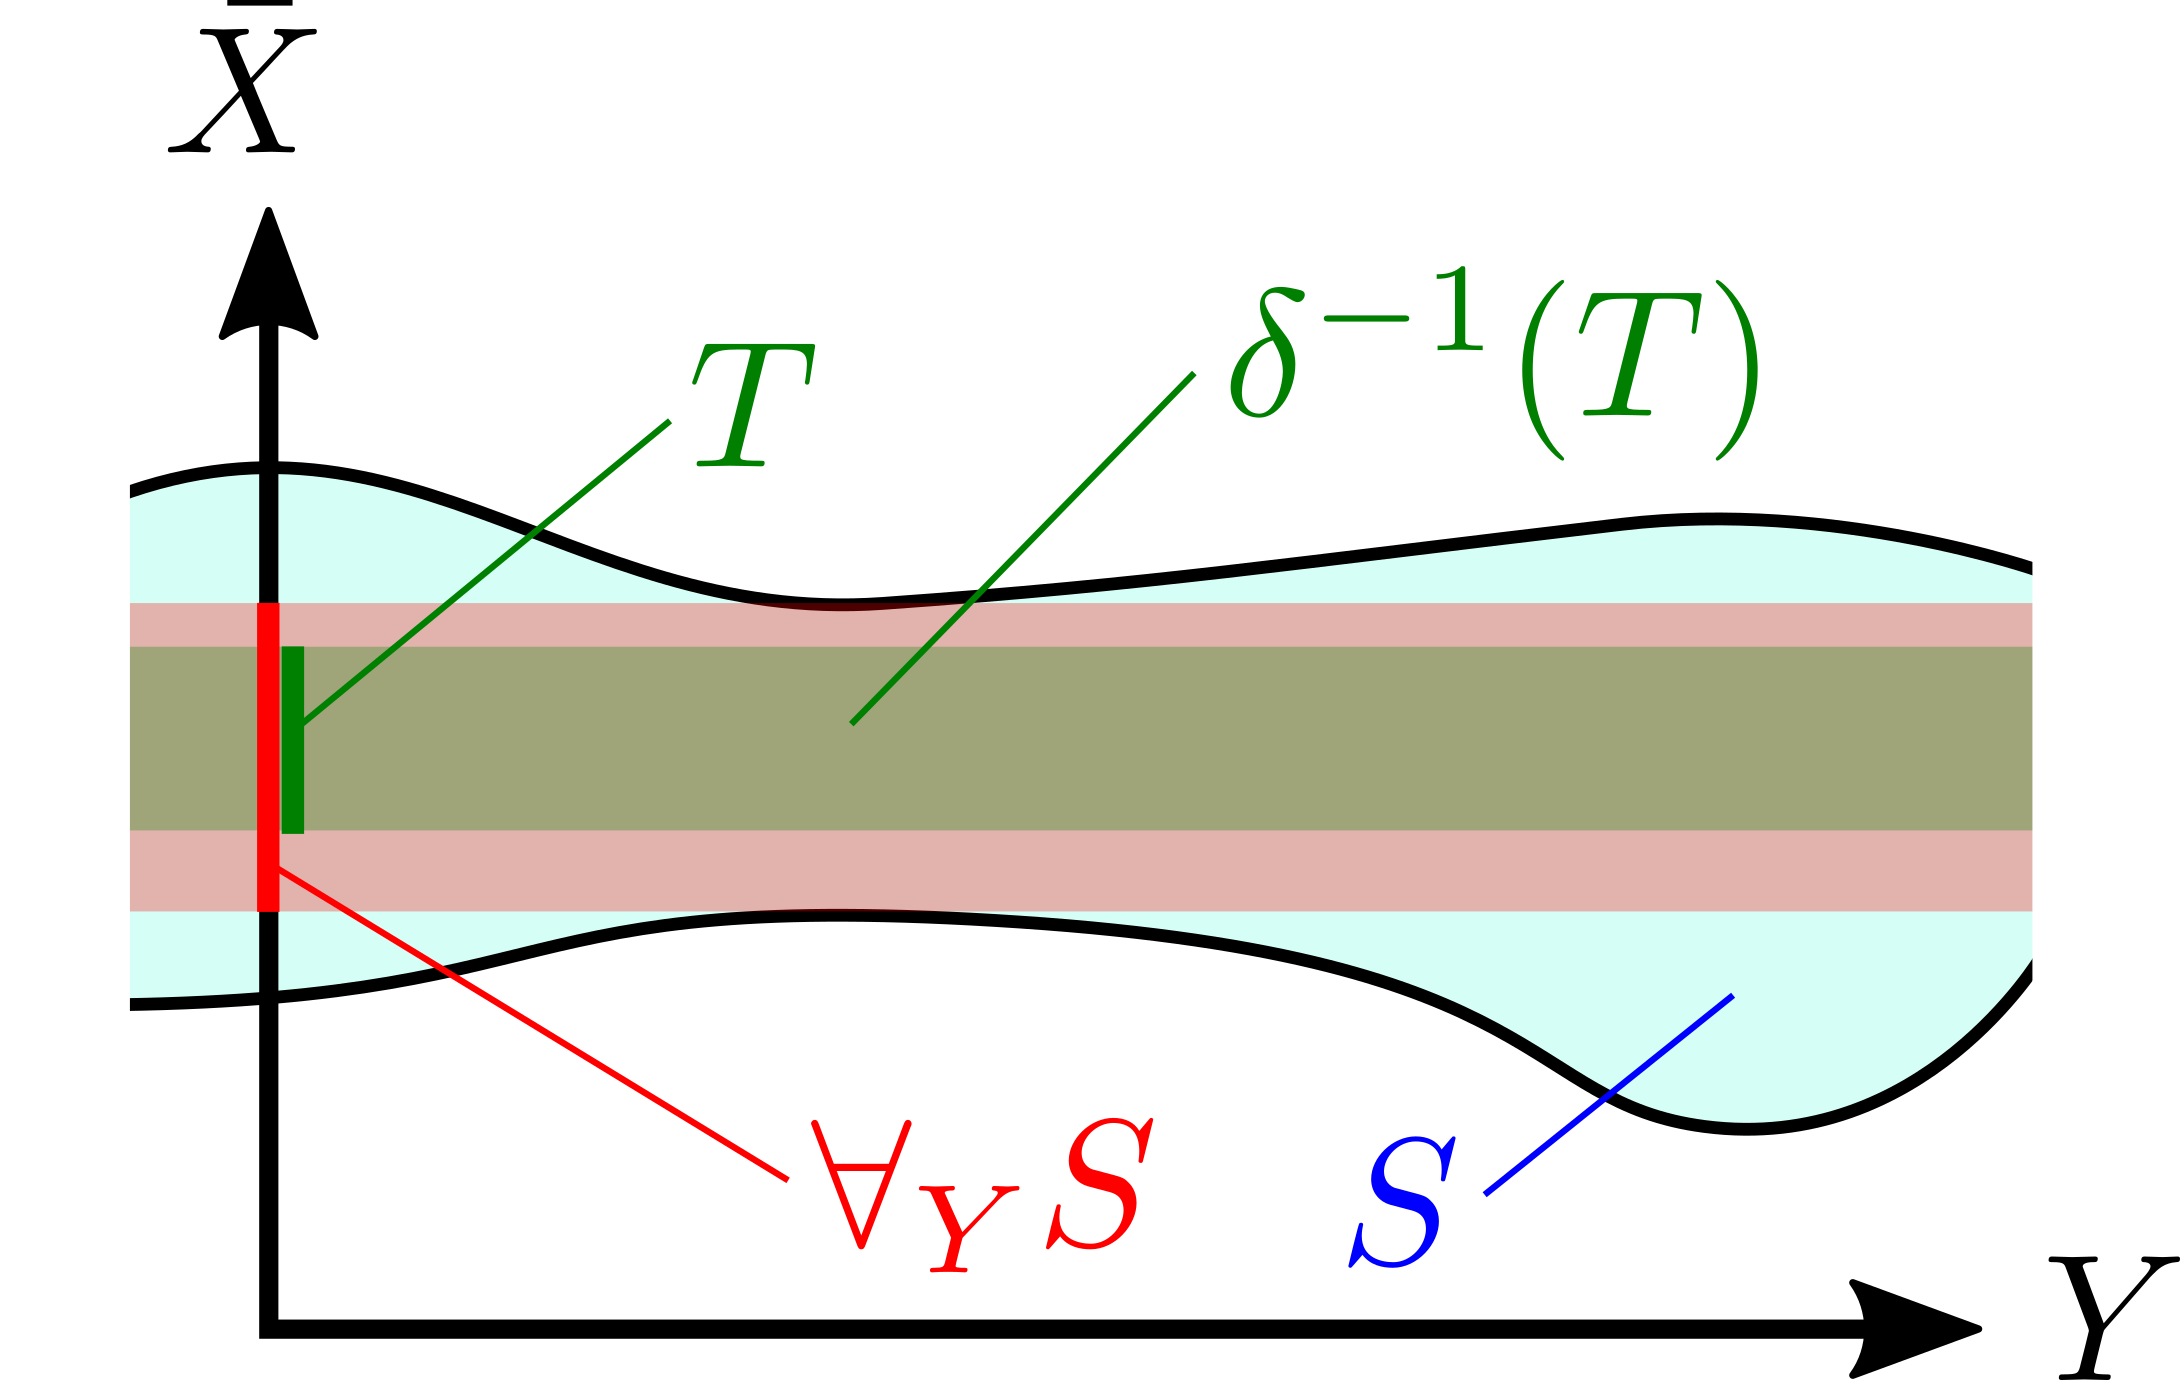
\includegraphics[scale=0.7]{Lawvere-cylindrification-forall.png}}}
\end{equation}

\subsection{$\wedge$ and $\Rightarrow$ as product-hom adjunction}

一个只有原子命题的逻辑系统是「静止」的,不能推出新的结论: 
\begin{eqnarray}
A & \qquad & A \nonumber \\
B & \quad \vdash \quad & B \\
C & \qquad & C \nonumber
\end{eqnarray}
但如果左边加多一个式子 $A \Rightarrow D$,则可以推出新的结论 $D$:
\begin{eqnarray}
\label{eqn:deduction}
A & \qquad & A \nonumber \\
B & \quad \vdash \quad & B \\
C & \qquad & C \nonumber \\
& \hspace*{-3em} {\color{red}A \Rightarrow D} \qquad & D \nonumber
\end{eqnarray}
换句话说,$\Rightarrow$ 算符 是逻辑引擎的「燃料」,没有它不能推动逻辑 inference 的过程。 

$\vdash$ 的功能和 $\Rightarrow$ 类似,但 $\vdash$ 是 \textbf{元逻辑} (meta-logic) 的符号,而 $\Rightarrow$ 是逻辑\textbf{之内}的算符。

在 (\ref{eqn:deduction}) 中,${\color{red} A \Rightarrow D}$ 导致了 $A \vdash D$ 的出现。

一般来说,$\Delta \Rightarrow \Gamma$ 就是 $\vdash$ 这个映射 对於 $\Delta$ 的一个 \emp{截面} (a restriction of the $\vdash$ map to the domain $\Delta$).  这一点很重要: 一个 map 作用在某些元素上,但这些元素 和那个 map 是「同类」的。 这其实是逻辑结构的一个 defining characteristic.

在 topos 里有一个很重要的 \emp{product-hom adjunction},  它说的是 $A \wedge B$ 和 $A \Rightarrow B$ 之间的邻接:
\begin{equation}
(A \times B) \rightarrow C \quad \simeq \quad A \rightarrow (B \rightarrow C)
\end{equation}
这在逻辑上 是见惯的,没有什么稀奇,它推论 $A \Rightarrow B$ 可以替代 $A \vdash B$.  由於 $\vdash$ 在我们的 AI 系统中是 \textbf{神经网络},这表示 神经网络中的「黑箱」知识可以「外在化」(externalize) 成 \textbf{逻辑命题},这一点 在智能系统中 是有关键的重要性,因为它表示 知识可以透过语言学习得到(虽然这也不是必需 范畴论 才可以看得出来。) 

\subsection{Classifying topos $\leftrightharpoons$ internal language}

问题是 witness 是什么?  例如「匙羹在杯内」是因为其他 视觉 propositions 得到的结论。 它是 true 这一点是重要的,但它的 ``intension'' 更重要。  或者说 proof 过程中处理的是 proof objects.  

这个 proof object 它除了是一件 syntactic 的东西之外还可以是什么?  或者说 map 的 \textbf{domain} 是命题,但被 map 映射的是 evidence?

想认识一个\textbf{范畴},最重要的是问: 它的 objects 是啥? 它的 morphisms 是啥? 

Lambek 给出的对应是:
\begin{itemize}
	\item types $\leftrightsquigarrow$ objects
	\item terms $\leftrightsquigarrow$ morphisms
\end{itemize}

We have the following transformations betweeen two formalisms:
\begin{equation}
\begin{tikzcd}[column sep = 20ex]
\boxed{\mbox{topos}} \; \mathcal{C}
\arrow[r, shift left, "\mbox{internal language}"]
& T \; \boxed{\mbox{type theory}}
\arrow[l, shift left, "\mbox{classifying topos}"]
\end{tikzcd}.
\end{equation}
In other words,
\begin{equation}
\mathcal{C} = \mathcal{C}\ell(T), \quad T = \mathrm{Th}(\mathcal{C}).
\end{equation}

\subsection{Yoneda lemma}

\begin{equation}
\nonumber
\mbox{\cc{米田 信夫}{Nobuo Yoneda} (1930-1996)} \quad 
\vcenter{\hbox{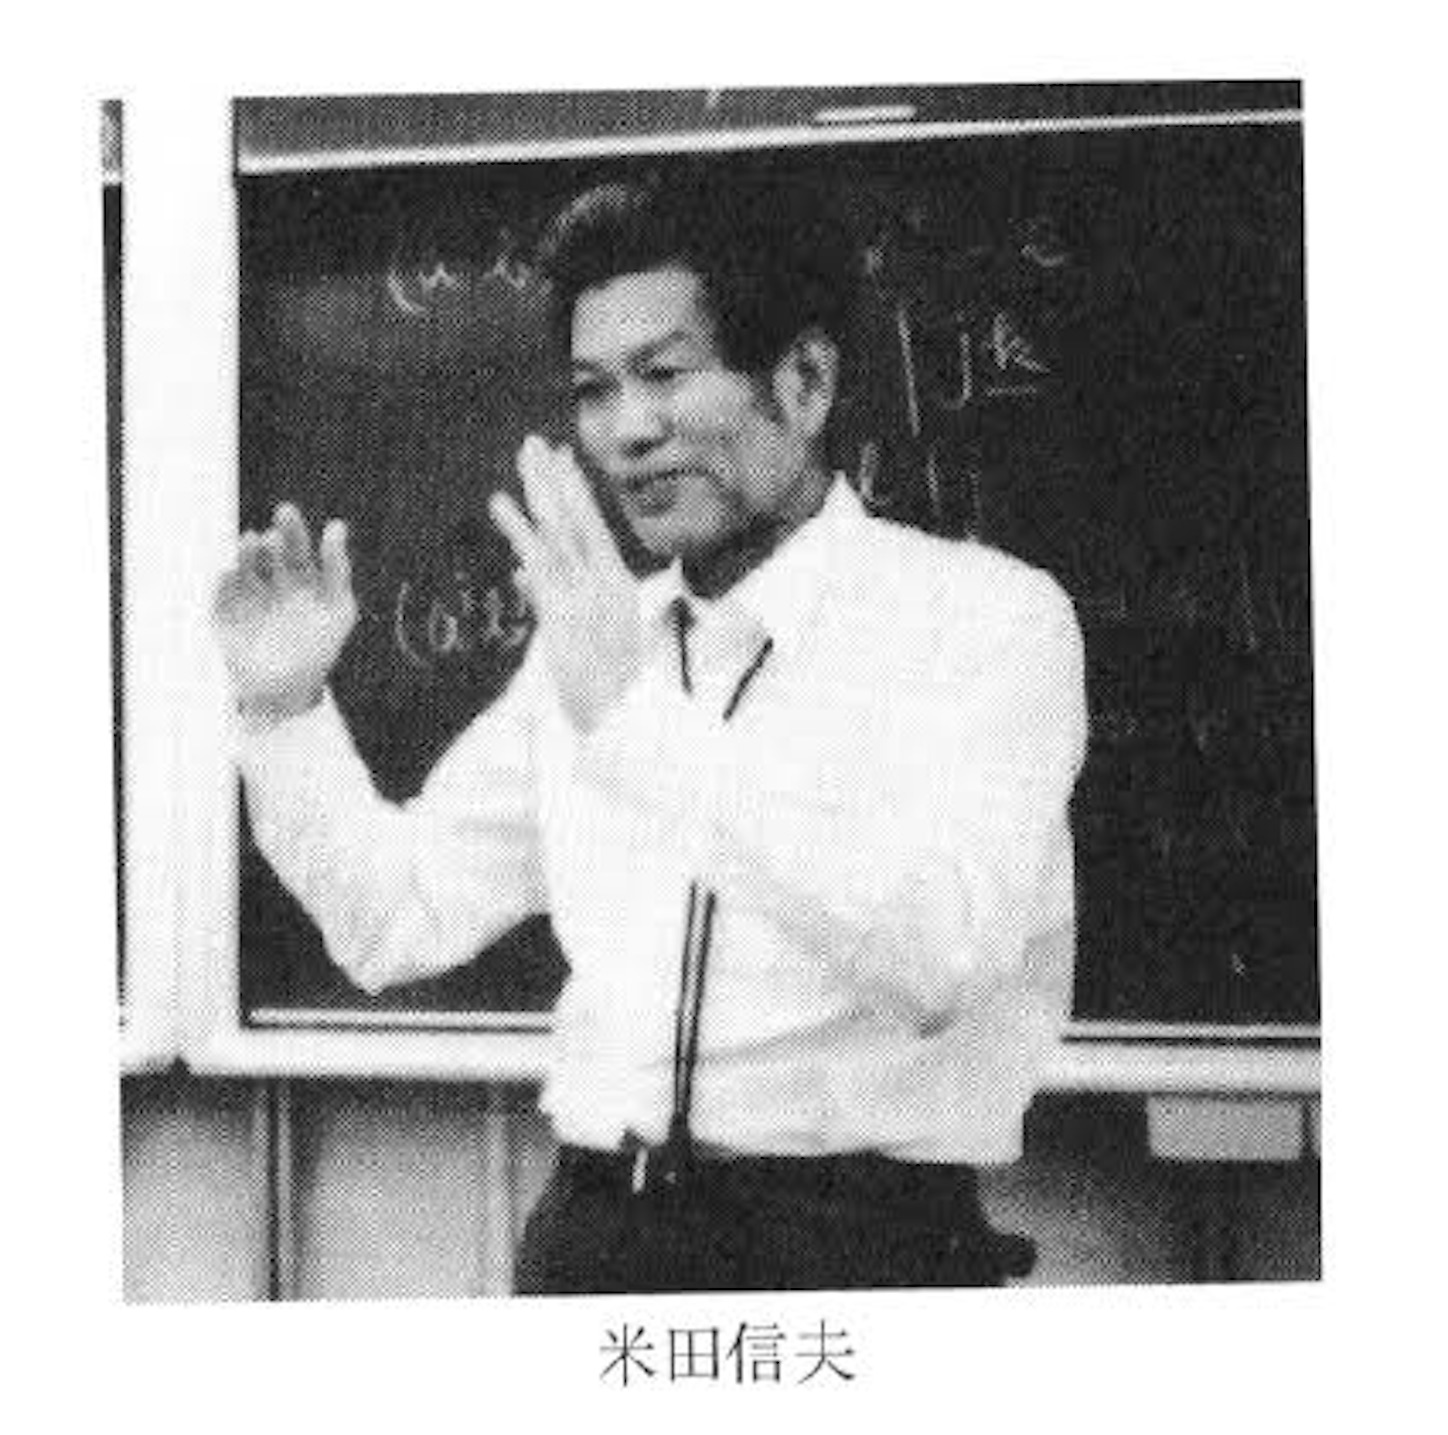
\includegraphics[scale=0.2]{Yoneda.jpg}}}
\end{equation}


在一个范畴 $\mathcal{C}$ 里面,考虑 其中一个物体 $A$ 到其他物体的 morphism, $A \rightarrow \bullet$.  这可以说是,透过 $A$「看」其他物体的方法。

\textbf{例:} 在 $\mathbf{Set}$ 里面,$1 \rightarrow X$ 是用 终点物体 1「看」其他物体,看到的是集合的 \textbf{元素}。

\textbf{例:} 映射 $\mathbb{R} \rightarrow X$ 是 空间 $X$ 中的 \textbf{曲线},可以说 $\mathbb{R}$「看到」曲线。

\textbf{例:} 在 ordered set $(\mathbb{R}, \le)$ 里面 物体 $0 \rightarrow x$ 可以「看到」$x$ 是不是 \textbf{positive}.

类似地,可以考虑 对偶 的情况,$\bullet \rightarrow A$ 是其他物体怎样「看」$A$ 的方法。

\textbf{例:} 在 $\mathbf{Set}$ 里面,$X \rightarrow 2$ 是其他物体「看」2 的方式,得到的是 $X$ 的\textbf{子集}, $\powerset(X)$. 

\textbf{例:} 在 $\mathbf{Top}$ 里面,2 包含一个 open set 和一个 closed set,$X \rightarrow 2$ 得出的是 $X$ 的\textbf{开子集},$\mathrm{Opens}(X)$.

A functor $X: \mathcal{A} \rightarrow \mathbf{Set}$ is \emp{representable} if $X \cong H^A$ for some $A \in \mathcal{A}$.

$H^A$ 的意思是 $\mathcal{A}(A, -)$, 这是一个集合。 

A \emp{representation of $X$} is a choice of an object $A \in \mathcal{A}$ and an isomorphism between $H^A$ and $X$. 

\emp{Yoneda embedding} of $\mathcal{A}$:
\begin{equation}
H_{\bullet}: \mathcal{A} \rightarrow [\mathcal{A}^{\mathrm{op}} , \mathbf{Set}]
\end{equation}

\begin{align}
\mbox{For each } A \in \mathcal{A} \mbox{, we have a functor} \quad
& \mathcal{A} \stackrel{H^A}{\longrightarrow} \mathbf{Set} \nonumber \\
\mbox{Putting them all together gives a functor} \quad
& \mathcal{A}^{\mathrm{op}} \stackrel{H^{\bullet}}{\longrightarrow} [\mathcal{A} , \mathbf{Set}] \\[10pt]
\mbox{For each } A \in \mathcal{A} \mbox{, we have a functor} \quad
& \mathcal{A}^{\mathrm{op}} \stackrel{H_A}{\longrightarrow} \mathbf{Set} \nonumber \\
\mbox{Putting them all together gives a functor} \quad
& \mathcal{A} \stackrel{H_{\bullet}}{\longrightarrow} [\mathcal{A}^{\mathrm{op}} , \mathbf{Set}] \nonumber
\end{align}

\begin{equation}
\begin{tikzcd}
\mathcal{A}^{\mathrm{op}} 
\arrow[r, bend left=30, "H_A"]
\arrow[r, bend right=30, swap, "X"]
\arrow[r, phantom, "\Downarrow"]
& \mathbf{Set}
\end{tikzcd}
\end{equation}

\emp{Yoneda lemma}:
\begin{equation}
[\mathcal{A}^{\mathrm{op}} , \mathbf{Set}] (H_A, X) \cong X(A)
\end{equation}

How sheaves gives rise to representables.

\subsubsection{Application: symmetric neural networks}

(这个可能是 Yoneda lemma 的一个应用,但我未详细检证)

The \textbf{Kolmogorov–Arnold representation theorem} states that every multivariate continuous function can be represented as a sum of continuous functions of one variable:
\begin{equation}
f(x_1,... ,x_n) = \sum_{q=0}^{2n}\Phi_{q} \left(\sum_{p=1}^n \phi_{q,p}(x_p) \right)
\end{equation}
It can be specialized to such that every symmetric multivariate function can be represented as a sum of (the same) functions of one variable:
\begin{equation}
\label{symmetric-functions}
f(x_1, ..., x_n) = g(h(x_1) + ... + h(x_n))
\end{equation}

Cayley's theorem:  Any group can be represented as a sub-group of a special group, namely the permutation group.

Any symmetric function can be represented as a sub-function of a special symmetric function, namely the sum.

\subsection{Model theory, functorial semantics}

We interpret formulas in a topos $\mathcal{E}$ by assigning each an \emp{extension}.  This is called \emp{internal} semantics.

\begin{equation}
\tikzmark{a1} a \tikzmark{c1} \; {\color{red}\cdot} \; \tikzmark{b1} b \longmapsto \llbracket \tikzmark{a2} a \rrbracket \tikzmark{c2} \; {\color{red}\cdot} \; \llbracket \tikzmark{b2} b \rrbracket
\begin{tikzpicture}[overlay, remember picture, distance=1.1cm]
\draw[->, out=45, in=135, transform canvas={shift={(4pt,15pt)}}] (a1.center) to (a2.center);
\draw[->, out=45, in=135, transform canvas={shift={(4pt,15pt)}}] (b1.center) to (b2.center);
\draw[->, out=-45, in=-135, transform canvas={shift={(6pt,-2pt)}}, red] (c1.center) to (c2.center);
\end{tikzpicture}
\end{equation}


\subsection{Generalized elements}

一个 逻辑命题 $\phi$ 可以看成是由 某论域 $A \stackrel{\phi}{\rightarrow} \Omega$ 的函数,其中 $\Omega = \{ \top, \bot \}$.

也可以说:命题 $\phi(x)$ 是真的,其中 $x$ 是 $A$ 的\emp{元素}。 In category theory, we use the terminal object $1$ to ``pick out'' elements of $A$, as follows:
\begin{equation}
1 \stackrel{x}{\rightarrow} A \stackrel{\phi}{\rightarrow} \Omega.
\end{equation}
In $\mathbf{Set}$, 任意一个由 1 出发的函数 $x: 1 \rightarrow A$ 可以直接看成是 $A$ 的「元素」。

但如果我们用另一个 论域 $C$ 取代 1,换句话说:
\begin{equation}
C \stackrel{x}{\rightarrow} A \stackrel{\phi}{\rightarrow} \Omega.
\end{equation}
这样的 $x: C \rightarrow A$ 叫作 $A$ 的 \emp{generalized element}.

另一个术语是: $C$ \emp{forces} $\phi(x)$, notation: $C \Vdash \phi(x)$.  这术语来自 Paul Cohen 为了解决 Continuum Hypothesis 而提出的 forcing 技巧,见 \S\ref{sec:forcing}.

另一个说法是: $\phi(x)$ is true \emp{at stage} $C$. (这术语来自 possible-world semantics)

\subsection{Internal vs external semantics}

假设 $\phi(\bullet)$ 是一个谓词,$\phi$ 的论域 (domain) 是 $A$.  例如 $\phi(x)$ 表示 $x$ 是男性,$x \in$ 人。  则 $\phi(x)$ 这个命题的 \emp{extension}(外延)就是在「人」的集合中属於「男性」的元素。 

知道了 $\phi$ 的 extension 就可以判断,对每一个 $x \in A, \phi(x)$ 的真假。  换句话说,提供了一种 \emp{interpretation} 的方法。 

The ``internal'' way to interpret type theory in a topos is where a formula $\phi$ in context $x_1: A_1, ... , x_n: A_n$ is interpreted as a \textbf{subobject} of $A_1 \times ... \times A_n$.

这个方法叫 \emp{internal semantics}.(注意 extension 的概念是 internal 的,有点混淆)

另一种方法是: 指定 哪些 generalized elements 符合某个 谓词。  后者叫 \emp{external semantics}:

\subsection{Kripke-Joyal / external semantics}

External semantics describe which generalized elements satisfy each formula.

Generalized element 的意思是 $I \stackrel{a}{\rightarrow} A \stackrel{\phi}{\rightarrow} \Omega$, 记作 $a \Vdash \phi$.

A generalized element satisfies a formula iff it is a member of the formula's \textbf{extension}.

\subsection{Cohen's method of forcing}
\label{sec:forcing}

在 数理逻辑/集合论 里,forcing 指的是一些 加在某 集合 $G$ 上的 \emp{条件},说某些 元素 属於 或不属於 $G$.  这些 条件 用逻辑表达,例如:
\begin{equation}
c = \{ 3 \in G, 57 \notin G, 873 \notin G \}
\end{equation}
is a condition.

例如,条件 $c$ 可以「强迫」集合 $G$ 里面至少有 100 个质数、或至少有 1万个质数。 记作 $c \Vdash P$, $P$ 是某个逻辑命题。

以下内容和 AGI 无关,但因为数学上有趣所以写一下。

Continuum hypothesis (CH):
\begin{equation}
2^{\aleph_0} = \aleph_1
\end{equation}
这是说: 连续统 $[0,1]$ 的基数 $2^{\aleph_0}$ 紧接在 可数集合的基数 之后。

1878 年,Cantor 提出 CH \\
1900 年,Hilbert 列出 连续统假设 为「23问题」的第一个 \\
\tab Hilbert 给出了一个证明,但里面有 bug \\
1938 年,G\"{o}del 证明 ZF + CH is consistent,换句话说:ZF cannot disprove CH \\
1963 年,Paul Cohen 证明 ZF cannot prove CH \\
\tab 他用的方法叫 ``forcing''
\begin{equation}
\mbox{Paul Cohen (1934-2007)} \quad \vcenter{\hbox{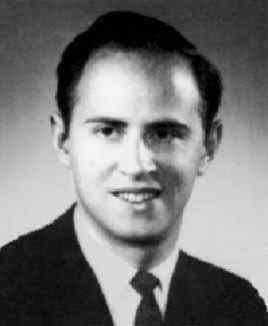
\includegraphics[scale=0.5]{Paul-Cohen.jpg}}}
\nonumber
\end{equation}

\subsection{Sheaves}

Sheaves capture the idea of ``indexing''.

Functors $\mathcal{C}^{\mathrm{op}} \rightarrow \mathbf{Set}$ are called \emp{pre-sheaves} on $\mathcal{C}$.

Pre-sheaf 要变成 sheaf 还需符合 sheaf condition,这是一种典型的 gluing condition, 意思是在 $U_i \cap U_j$ 这些重合的邻域上,presheaf 的 sections 是\textbf{一致}的。 

当 $\mathcal{C}^{\mathrm{op}}$ = topology of open sets 时,我觉得下图特别容易理解:
\begin{equation}
\vcenter{\hbox{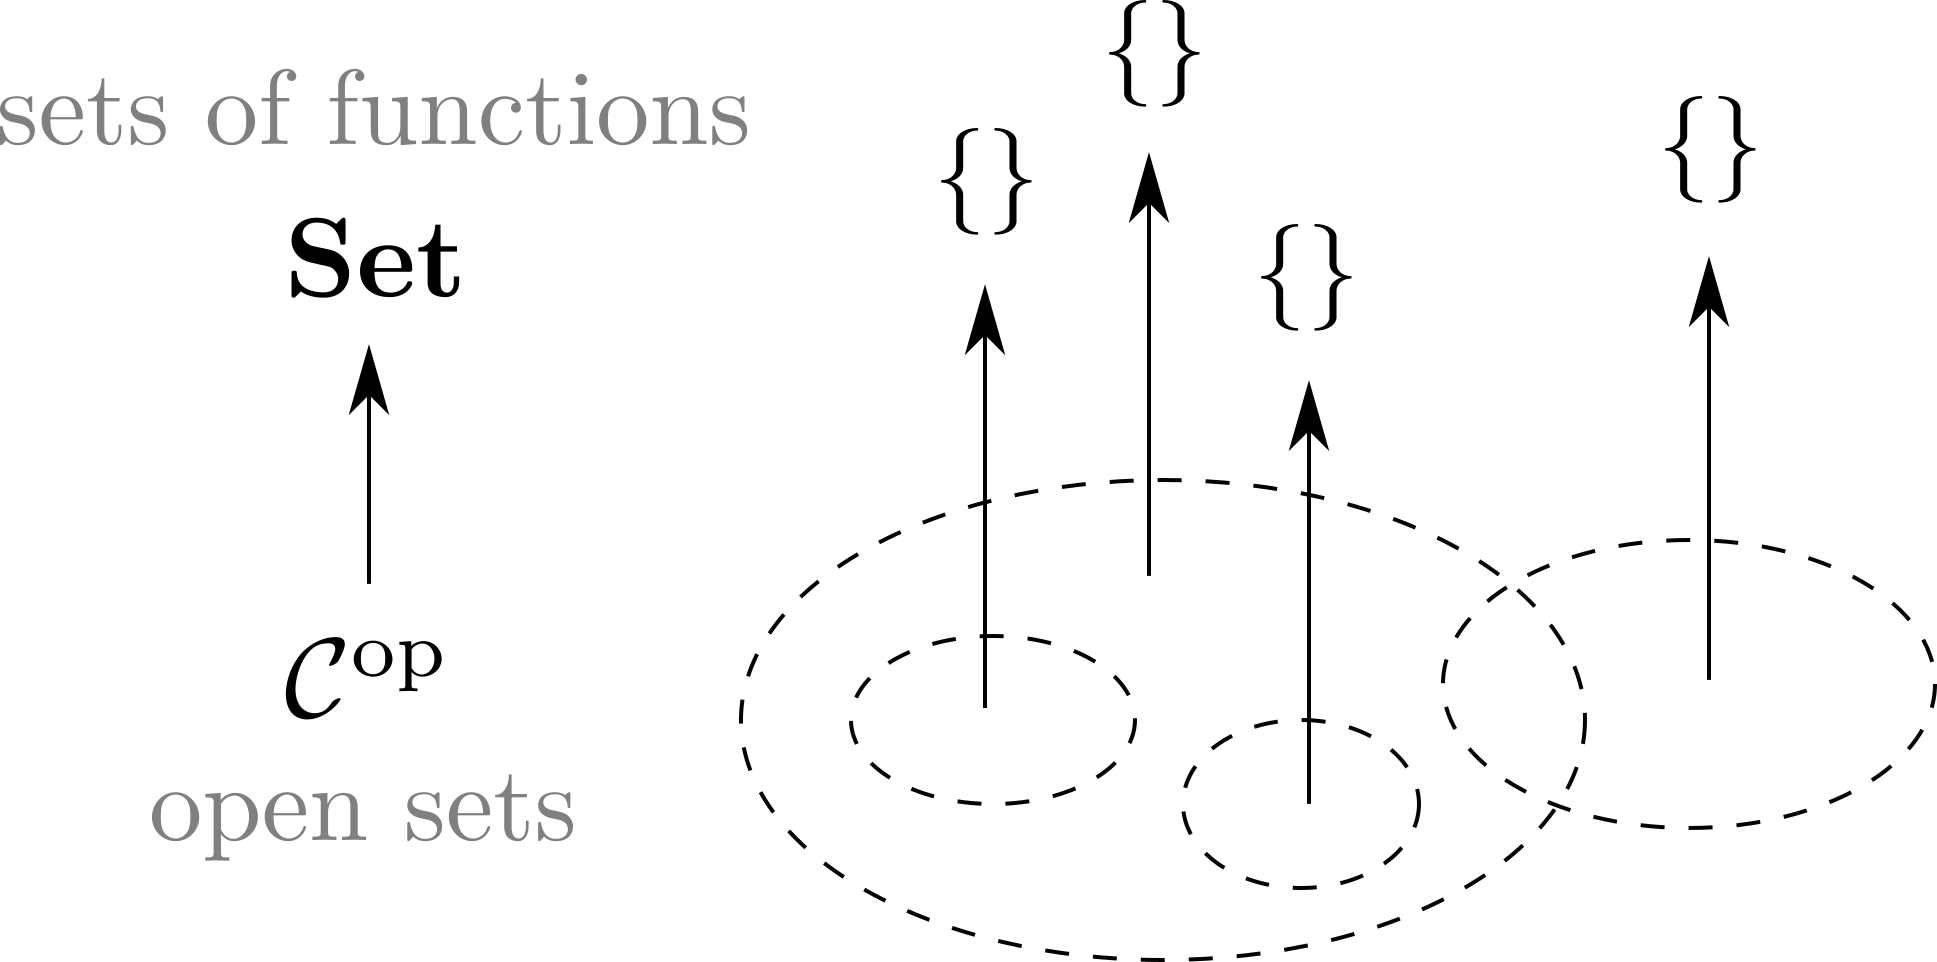
\includegraphics[scale=0.7]{sheaf.png}}}
\end{equation}

Some $\mathbf{Set}$-valued functors are \emp{representable}, ie, isomorphic to a hom-functor.

For an object $S$ of a category $\mathcal{C}$, the functor
\begin{equation}
H^S : \mathcal{C} \rightarrow \mathbf{Set}
\end{equation}
sends an object to its set of generalized elements of shape $S$.  The functoriality tells us that any map $A \rightarrow B$ in $\mathcal{C}$ transforms $S$-elements of $A$ into $S$-elements of $B$.  For example, taking $\mathcal{C} = \mathbf{Top}$ and $S = S^1$, any continuous map $A \rightarrow B$ transforms loops in $A$ into loops in $B$.

In logic, the category of predicates can be regarded as a sheaf over its domain $\mathrel{\substack{\mathbf{Pred}\\\downarrow\\\mathbf{Set}}}$.

我暂时还不太清楚 sheaf 理论对 AI 来说有什么重大意义。 

\subsection{Kleene realizability}

\underconst

\section{Intuitionistic logic}

In 1933, G\"{o}del proposed an interpretation of intuitionistic logic using possible-world semantics.

In topos theory $A \Rightarrow B$ is adjoint (via the hom-product adjunction) to $A \vdash B$, which is ``okay'' because it is independent of which implication (material or strict) we are using.

\subsection{Heyting algebra}

\begin{equation}
\mbox{Arend Heyting (1898-1980)} \quad 
\vcenter{\hbox{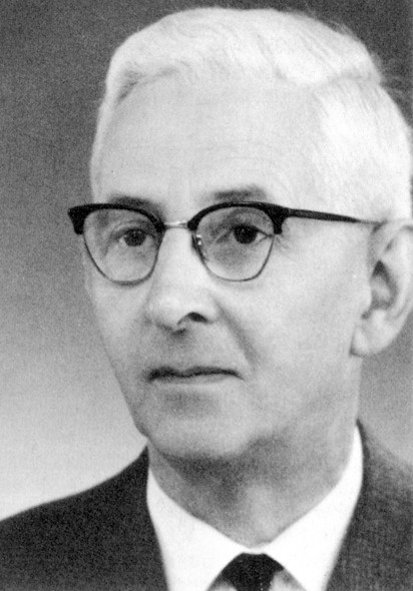
\includegraphics[scale=0.3]{Heyting.jpg}}}
\end{equation}
1930 年,Heyting 给出了 constructive mathematics 的一种 axiomatization, called \emp{intuitionistic logic} (IL).  Heyting algebra 是一种 IL 的 \emp{代数模型},正如 Boolean algebra 是 经典逻辑的 代数模型。 

Heyting algebra is to intuitionistic logic what Boolean algebra is to classical logic.

例如,以下的 \emp{拓樸}模型 和 \emp{格} (lattice) 模型,都是 Heyting algebra 的模型:
\begin{equation}
\boxed{
\begin{aligned}
\mbox{下雨} & \\
& \hspace*{1em} \boxed{\mbox{草地湿}} \\
& \boxed{\mbox{没得打网球}} \; 
\end{aligned}
} \quad \quad
\vcenter{\hbox{
\begin{tikzpicture}[scale=0.8]
\node[label={[xshift=0em, yshift=-0.5em]\mbox{下雨}}] (a) at (1,0) {\textbullet};
\node[label={[xshift=-0.5em, yshift=-2em]\mbox{草地湿}}, swap] (b) at (0,-2) {\textbullet};
\node[label={[xshift=1.5em, yshift=-2em]\mbox{没得打网球}}, swap] (c) at (2,-2) {\textbullet};
\draw[-,shorten <=-10pt, shorten >=-10pt] (a) to (b);
\draw[-,shorten <=-10pt, shorten >=-10pt] (a) to (c);
\end{tikzpicture}
}}
\end{equation}
两者之间是等价的,起源於 \emp{Stone duality} (every Boolean algebra is isomorphic to a topology of open sets),其后再被推广到 \emp{Priestley} 拓扑对偶 等,都是大同小异的。

注意: $\mbox{下雨} \Heytingarrow \mbox{草地湿}$ 是 Heyting implication,这个 $\Heytingarrow$ 的存在 并不是因为「下雨」的\textbf{真值} 比「草地湿」的\textbf{真值 小}。 

The Heyting implication $a \Heytingarrow b$ exists for all elements $a, b, x$ such that:
\begin{equation}
x \le (a \Heytingarrow b) \quad \mbox{iff} \quad (x \wedge a) \le b.
\end{equation}

Every Boolean algebra can be a Heyting algebra with the material implication defined as usual: $a \Rightarrow b \equiv \neg a \vee b$.

可以用以下例子说明 Heyting implication $\Heytingarrow$ 的定义:
\begin{equation}
\forall X. \quad X \subseteq (\highlight{\mbox{下雨} \Heytingarrow \mbox{草地湿}}) \quad \mbox{iff} \quad (X \wedge \mbox{下雨}) \subseteq \mbox{草地湿}
\end{equation}
\begin{equation}
\vcenter{\hbox{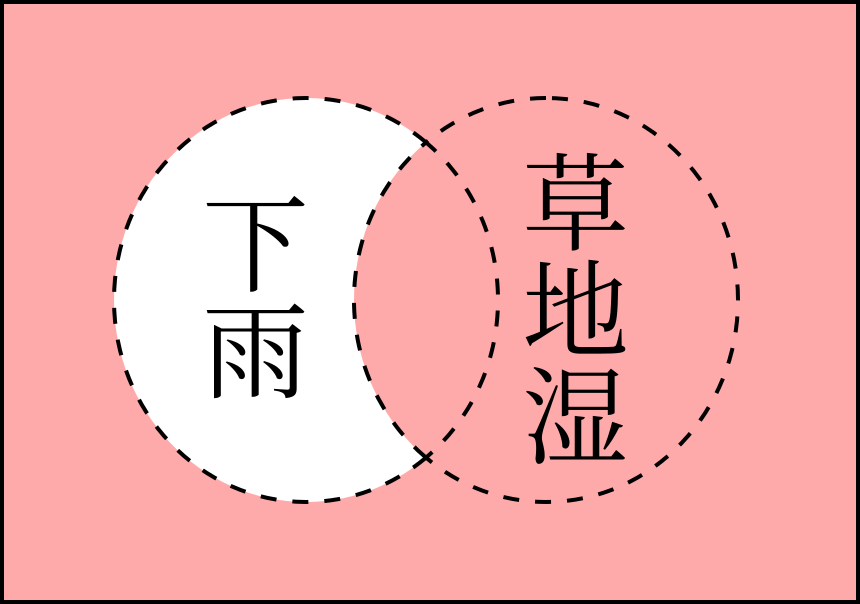
\includegraphics[scale=0.8]{topology-Heyting-rain-wet.png}}}
\end{equation}

经典逻辑的 $\Rightarrow$ 和 直觉主义逻辑 $\Heytingarrow$ 只有 在\textbf{边界}上的 微小差异:
\begin{align}
\mbox{classical $A \Rightarrow B$} \qquad & \qquad
\mbox{Heyting $A \Heytingarrow B$} \nonumber \\
\vcenter{\hbox{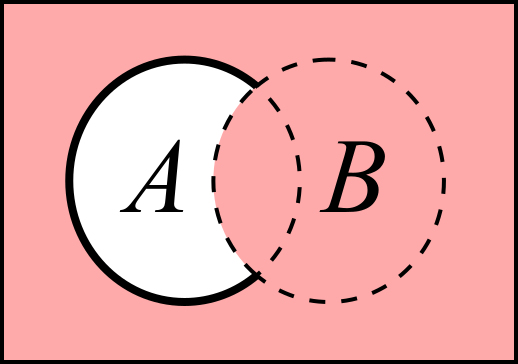
\includegraphics[scale=1]{topology-classical-implication.png}}}
\qquad & \qquad
\vcenter{\hbox{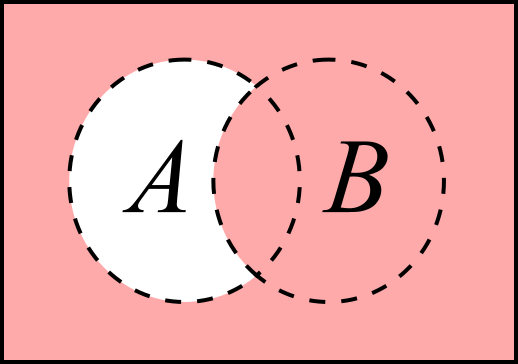
\includegraphics[scale=1]{topology-Heyting-implication.png}}}
\end{align}
无论是何种逻辑,以下的两边是 \textbf{等价}的:
\begin{align}
\mbox{$A \Rightarrow B$} \quad & \Longleftrightarrow \quad \mbox{$A \vdash B$ or $A \subseteq B$} \\
\vcenter{\hbox{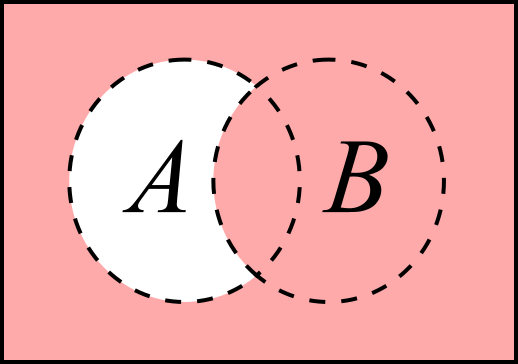
\includegraphics[scale=1]{topology-Heyting-implication.png}}}
\quad & \Longleftrightarrow \quad 
\vcenter{\hbox{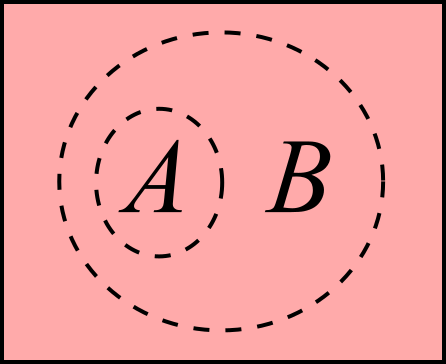
\includegraphics[scale=1]{topology-implication-2.png}}}
\end{align}
这可以看成是 将白色部分不断 缩小并「消灭掉」的结果。 

根据 Stone duality, 既然可以用 Boolean 或 Heyting algebra 做逻辑推导,因此 也可以用 toplogy of (open) sets 做逻辑推导。 其根据的就是:
\begin{equation}
A \vdash B \quad \mbox{和} \quad A \subseteq B
\end{equation}
之间的 等价。

这种 topology 可以视为 \textbf{truth table} 的一种形式,如下图所示,每个\textbf{区域}代 表 真值表的\textbf{一行}:
\begin{equation}
\begin{tabular}{|c|c|c|c|}
	\hline 
	{\color{red}$A$} & {\color{red}$B$} & {\color{red}$C$} & \# \\ 
	\hline 
	$\top$ & $\top$ & $\top$ & 1 \\ 
	\hline 
	$\top$ & $\top$ & $\bot$ & 2 \\ 
	\hline 
	$\top$ & $\bot$ & $\top$ & 3 \\ 
	\hline 
	$\top$ & $\bot$ & $\bot$ & 4 \\ 
	\hline 
	$\bot$ & $\top$ & $\top$ & 5 \\ 
	\hline 
	$\bot$ & $\top$ & $\bot$ & 6 \\ 
	\hline 
	$\bot$ & $\bot$ & $\top$ & 7 \\ 
	\hline 
	$\bot$ & $\bot$ & $\bot$ & 8 \\ 
	\hline 
\end{tabular}
\quad \Longleftrightarrow \quad
\vcenter{\hbox{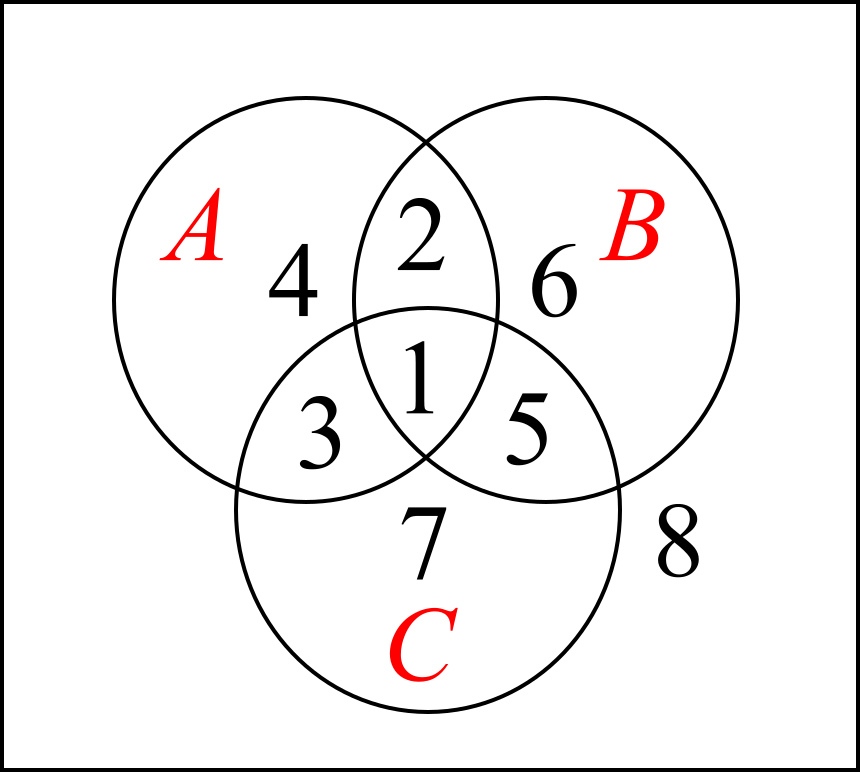
\includegraphics[scale=1]{topology-ABC.png}}}
\end{equation}

之所以讲这么多,目的是想说明,Heyting algebra 和我们熟悉的 Boolean algebra 其实有很多共通点。 

另一点发现是,在 \S\ref{sec:material-implication} 所说的 material implication 问题,在 intuitionistic logic 里仍然存在。

In a topos $\mathbb{E}$, the subobject $\mathrm{Sub}_{\mathbb{E}}(A)$ is a \emp{poset} that admits \emp{Heyting implication}.  

Using Kripke semantics, the Heyting arrow $\rightarrow$ can be defined by:
\begin{equation}
k \Vdash A \rightarrow B \quad \Leftrightarrow \quad \forall \ell \ge k \; (\ell \Vdash A \Rightarrow \ell \Vdash B)
\end{equation}

Whereas the ``fish-hook'' \emp{strict implication} can be defined as ``A implies B necessarily'':
\begin{equation}
A \strictif B \quad \equiv \quad \square (A \Rightarrow B) 
\end{equation}

The two can be regarded as equivalent via:
\begin{equation}
\begin{aligned}
k \Vdash \square (A \Rightarrow B) \quad \Leftrightarrow \quad & \forall \ell \ge k \; (\ell \Vdash (A \Rightarrow B)) \\
\quad \Leftrightarrow \quad & \forall \ell \ge k \; (\ell \Vdash A \Rightarrow \ell \Vdash B)
\end{aligned}
\end{equation}

问题是将 Heyting implication 定义 by possible worlds semantics 有什么好处?  从 machine learning 角度可能更合理。  但其实也好像包含 classical implication 所以是循环的?  

根据 topos 理论,Heyting implication 的出现是因为 sub-objects 的 Heyting algebra.  但我希望 implication arrow 纯粹是因为 BHK interpretation 而出现的。 

Heyting implication 的问题是它产生自 sub-object 概念。 Material truth will cause an implication to exist.  What does that mean?  

\section{Modal logic}

Modalities are often conceived in terms of variation over some collection or \textbf{possible worlds}.

A modal operator (such as $\square$) in the category $\mathbf{Sheaf}(X)$ is a \emp{sheaf morphism} $\square: \Omega \rightarrow \Omega$ satisfying 3 conditions, $\forall U \subseteq X$ and $p, q \in \Omega(U)$:
\begin{equation}
\begin{aligned}
& \mbox{a)} \quad p \le \square (p) \\
& \mbox{b)} \quad (\square ; \square) (p) \le \square (p) \\
& \mbox{c)} \quad \square (p \wedge q) = \square (p) \wedge \square (q)
\end{aligned}
\end{equation}

\subsection{Possible-world semantics}

Possible-world semantics is also called \emp{intensional semantics}, as opposed to \emp{extensional semantics} where truth values are directly assigned to propositions.  Does this idea jibe with the other definition of ``intension'', ie, as opposed to Leibniz extensionality and also related to intensional logic?

\begin{equation}
\nonumber
\mbox{Saul Kripke (1940-)} \quad 
\vcenter{\hbox{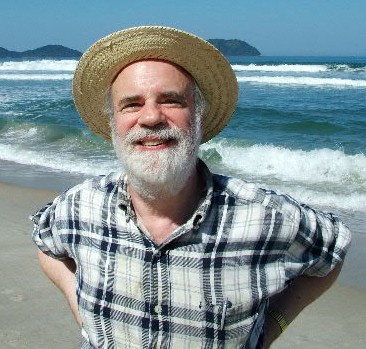
\includegraphics[scale=0.5]{Kripke.jpg}}}
\end{equation}

\subsection{Computer implementation of possible worlds}

要詮釋 modal logic,需要引入 frame $F = \langle W, R, D, H \rangle$, 其中:
\begin{itemize}
	\item $W$ = set of possible worlds = $\{ w_1, w_2, ... \}$
	\item $R$ = a relation between worlds, $w_i R w_j$
	\item $D$ = domain of first-order objects
	\item $H: W \rightarrow \powerset(D)$, for each world specify a subset of objects
\end{itemize}

To interpret formulas with $\square$:
\begin{equation}
M \Vdash \square A \; [w] \quad \Leftrightarrow \quad \forall w' \succeq w. \; M \Vdash A \; [w']
\end{equation}
這牽涉到要 quantify over all $w$'s.

重點是 inference 需要什麼 data?

顯然需要決定在某 $w$ 中 $p$ 是否成立,甚至需要判斷 $\forall w. p [w]$.

後者似乎需要將所有 有關的可能世界(或至少是其 summary)放到 working memory 再 quantify.  

\subsection{Intensional vs extensional}

``Beethoven's 9th symphony'' and ``Beethoven's choral symphony'' has the same \emp{extension} but different \emp{intensions}.

\subsection{Intensional logic}

Possible-world semantics is also called \emp{intensional semantics}, as opposed to \emp{extensional semantics} where truth values are directly assigned to propositions.

Logic terms differ in intension if and only if it is \textbf{possible} for them to differ in extension.  Thus, \emp{intensional logic} interpret its terms using possible-world semantics.

\subsection{Strict implication}
\label{sec:strict-implication}

\subsubsection{The problem of ``material implication''}

Material implication 的意思是「实质蕴涵」,亦即是说 $A \Rightarrow B$ 等价於 $\neg A \vee B$,其真值表如下:

\begin{equation}
\label{eqn:implication-truth-table}
\begin{tabular}{|c|c|c|}
\hline 
$A$ & $B$ & $A \Rightarrow B$ \\ 
\hline \hline 
0 & 0 & 1 \\
\hline 
0 & 1 & 1 \\ 
\hline 
1 & 0 & 0 \\ 
\hline 
1 & 1 & 1 \\ 
\hline 
\end{tabular} 
\end{equation}

Material implication 的概念向来很有争议,例如,当前提是错误时,它永远是真的: 
\begin{equation}
\mbox{瑞士在非洲} \Rightarrow \mbox{猪会飞}
\end{equation}

\begin{center}
\rule{0.8\textwidth}{1pt}
\end{center}

透过观察 truth table 可以发现,它的每一列 其实代表一个 \emp{可能世界},这些 可能世界 是不会 同时发生的。 换句话说,material implication 和 strict implication 本来是一样的,只是前者将 可能世界 的语义 隐蔽到「幕后」。 

For strict implication to make sense, it is always necessary to invoke possible-world semantics.  A strict implication is always \emp{learned} from numerous examples from experience, in accord with the philosophical tradition of ``empiricism''.

Strict implication is equivalent to material implication over multiple instances.  The truth table of material implication agrees with the functional interpretation of implication.  

\section{Fuzzy logic}
\label{sec:fuzzy-logic}

\begin{equation}
\nonumber
\mbox{Lotfi Zadeh (1921-2017)} \quad 
\vcenter{\hbox{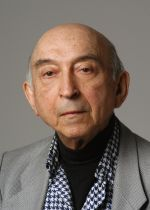
\includegraphics[scale=2.5]{Zadeh.jpg}}}
\end{equation}
Iranian-Jewish

首先是 implication 的问题,fuzzy implication 并不对应於 material implication in Boolean algebra.

另外有个问题就是要考察一下 fuzzy truth value 在各种情况下的正确性。 

例如假设 set 里面有 fuzzy proposition 的「证明」\\
又或者「人类」的集合是「有人类」这个命题的证明 \\
而,「数学家」作为「人类」的子集,等於命题「所有人都是数学家」的证明 \\
而这和 fuzzy value 是一致的

但为什么「John 是人」这个命题有点怪怪的? \\
如果它有 fuzzy value,应该是某集合的子集 \\
有些元素证明 John 是人,有些证明他不是人 \\
或者是 John 的\emp{属性}的集合? \\
而其中有些属性 imply 他是人? \\
或者有些属性 $\subseteq$ 人的属性?

还有这跟 ``Marilyn Monroe is sexy'' 是不是一致?
Marilyn 的所有属性集合,其中 imply sexy 的 subset \\
还是 sexy 的所有属性集合,其中 Marilyn 也有的?

Sexy(marilyn), Human(john), vs Human(Mathematicians).


What kind of mapping does this require?

\subsection{Fuzzy implication}
\label{sec:fuzzy-implication}

Implication 能不能 generalize 到 fuzzy logic 的情况?

\subsection{Fuzzy functions?}

What are fuzzy functions?

\section{Homotopy type theory (HoTT)}

\begin{equation}
\nonumber
\mbox{Vladimir Voevodsky (1966-2017)} \quad 
\vcenter{\hbox{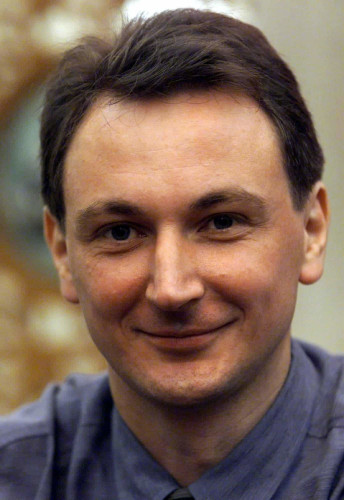
\includegraphics[scale=0.25]{Voevodsky.jpg}}}
\end{equation}

HoTT 的中心思想是将 types 看成是某些 空间 (spaces),而这些空间可以被赋予 topological 特别是 homotopy 结构。 在 homotopy 而言,关键是 将 type $A$ 里面两个元素的 \textbf{相等} $\mathrm{id}_A$ 看成是 homotopy 的 \textbf{path}.

\subsection{Why HoTT may be useful}

在 topos 上 $A \subseteq B$ 或 $a \in A$ 是一种 subset 关系,或者可以说是 topological 关系。  在计算机上,将这个 topology 赋予更多「空间」的特性,例如 vector space, metric space 等,似乎会是很 powerful 的。 

但问题是: 如果 $A$ 是 拓扑空间中某个(形状已知的)region,而 entity $a$ 的位置也是知道的,则 $a \in A$ 这个命题的真假 也立即可以知道。 但这是非常有问题的,例如「$e \in?$ 无理数」这个命题,必需复杂的证明,而不是瞬间可以判断。 又或者「OJ Simpson $\in?$ 杀人凶手」。

换句话说,似乎不可能将 命题空间 实现成某种有 \textbf{具体位置}的空间。  因此 $a \in A$ 这种命题,似乎 只能够表述成 ordered pair $(a, A)$,然后用\textbf{代数方法} 模拟 abstract topology.  这 其实就是我在 (\ref{eqn:brutal-syntactic-method}) 提到的「粗暴」syntactic 方法。 

挽救「位置空间」的一个办法是: 容许 OJ Simpson $\in$「黑人、男性、演员、球员」等,但保证他不属於其他(未被验证的)集合,后者是\textbf{未知}的。 但这样导致要 验证 潜在无穷多个集合,并不可行。

除非在 逻辑空间中 预先保证 每个集合 \textbf{并不相交},而如果 $x \in A \; \wedge \; x \in B$,则 设定 $x_1 \in A, \; x_2 \in B, \; x_1 = x_2$, and $x_1, x_2$ are \textbf{path-connected}.  所以这需要用到 HoTT.

暂时 仍未知道 这种做法 是不是比「粗暴」法更有效率。 

根据 paths 可以有如下的 topological「变形」:
\begin{equation}
\vcenter{\hbox{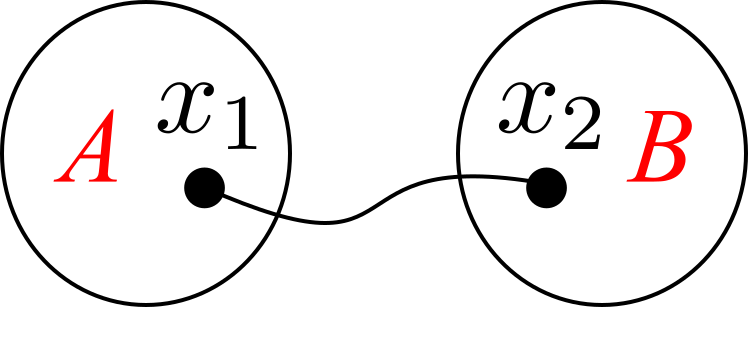
\includegraphics[scale=0.9]{path-morphing-1.png}}}
\quad \Longleftrightarrow \quad
\vcenter{\hbox{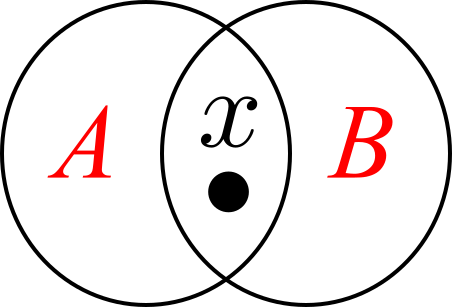
\includegraphics[scale=0.9]{path-morphing-2.png}}}
\end{equation}
但右边 仍是会出现 $x \in A$ accidentally 导致 $x \in B$ 的情况。

如果 neural network map $F$ 的对象不是 ordered pairs ($x \in A$), 可以是什么?  A \textbf{proposition} can be regarded as a set of points $x_i$ connected by paths.  

\subsection{HoTT levels}

\begin{equation}
\begin{tabular}{|c|c|}
	... & ... \\ 
	\hline 
	2 & 2-groupoids \\ 
	\hline 
	1 & groupoids \\ 
	\hline 
	0 & sets \\ 
	\hline 
	-1 & (mere) propositions \\ 
	\hline 
	-2 & contractable spaces \\ 
	\hline 
\end{tabular} 
\end{equation}

\subsubsection{Truncation}

$||A||$ is a way to obtain the \textbf{truth value} of a type $A$, known as \textbf{truncation}.  For Voevodsky, the truth value is always binary, the type of ``mere propositions''.  I propose that it can be generalized such that, on HoTT level 0, it provides the \textbf{fuzzy} truth value $\in [0,1]$.

\subsection{What is homotopy?}

\subsection{Univalence axiom}

在 HoTT 的 set 的层次,``='' 是一个 predicate, 根据我的理论可以看成是 fuzzy predicate.

如果我没理解错误,univalence axiom 的意思 似乎是将 = 的 fuzzy truth value「强制」成 binary.

\section{Transfer to deep learning}

这一节讨论 如何将上面提到的 logic structure 转移到 深度学习的 神经网络 (neural network, NN)。  一般来说,很难将 额外的结构 impose 在 神经网络上,因为 NN 本身已经有很 ``rigid'' 的结构。 在这方向上成功的例子是 CNN (convolutional NN),其中 convolution $f * g$ 是由 ``weight sharing'' 模拟。 但除此之外,一般很难在 NN 上添加结构。

\emp{Symmetric NN} 是一种 在输入变量的 \textbf{置换}下 不变 (permutation invariant) 的神经网络。 其解决 办法 是利用以下的 函数形式:
\begin{equation}
f(x_1, ..., x_n) = g(h(x_1) + ... + h(x_n))
\end{equation}
\begin{equation}
\vcenter{\hbox{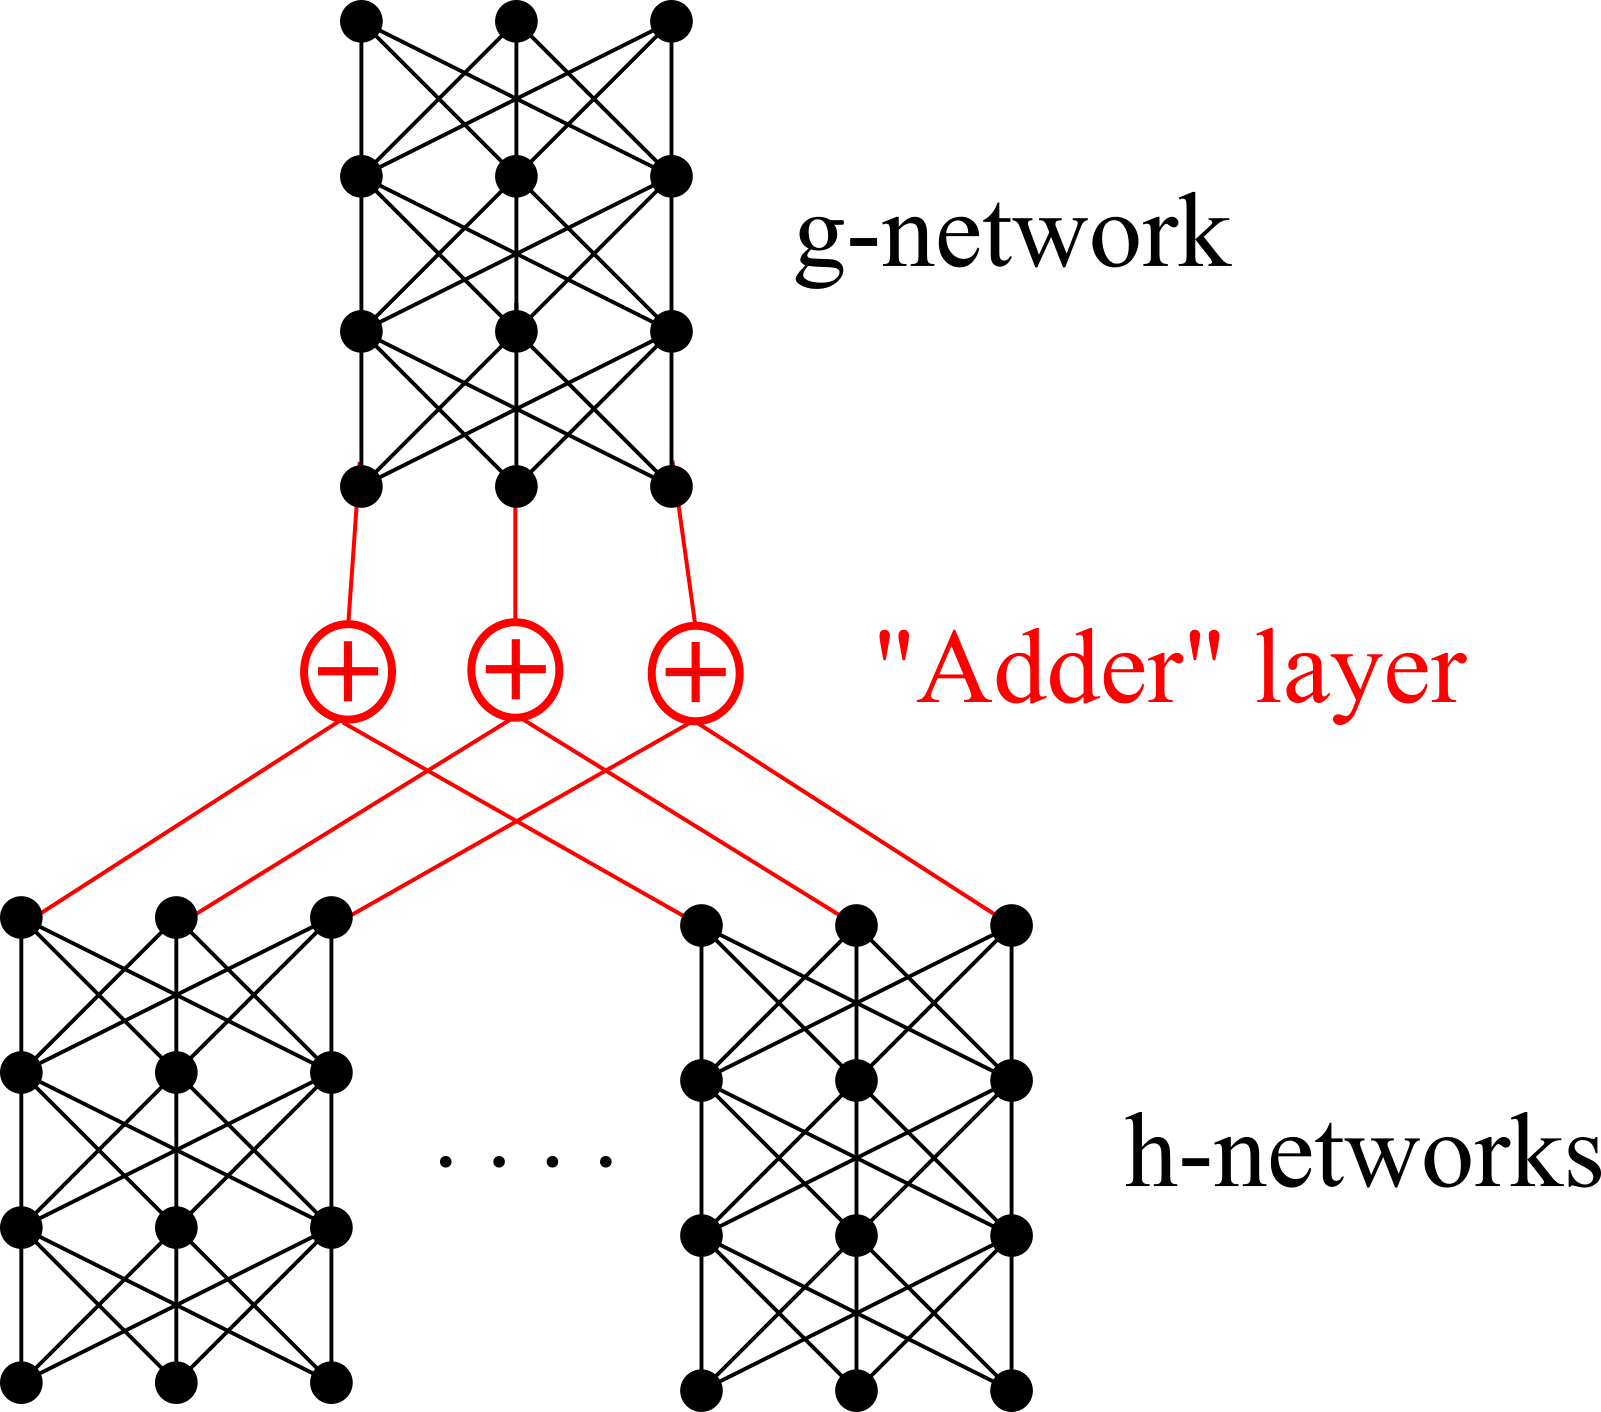
\includegraphics[scale=0.5]{g-and-h-networks.png}}}
\end{equation}
注意在这个方案下,NN 是以 ``black box'' 作为 building blocks; 内部结构不变。 

范畴论 的好处是,将一切用 morphisms, compositions, pullbacks, adjunctions, 等 表示; 这种做法 很容易用 NN implement.

\subsection{Propositional aspect}

在命题逻辑的层次上,我选择了最简单的特性,亦即是命题之间的 commutativity:
\begin{equation}
\begin{aligned}
A &\wedge B & \equiv && B & \wedge A \\
\mbox{\cc{下雨}{it's raining}} &\wedge \mbox{\cc{失恋}{lovesick}} & \equiv && \mbox{\cc{失恋}{lovesick}} &\wedge \mbox{\cc{下雨}{it's raining}}
\end{aligned}
\end{equation}
但我没有 fully exploit Heyting algebra or Boolean algebra 的结构,因为可以预见 将来是会 推广到 fuzzy-probabilistic logic,而后者的结构只需要 $\wedge$ 和 $\Rightarrow$,和 binary logic 有些不同(迟些解释....)

\subsection{Predicate aspect}

目前,一般的深度学习模型是比较 简单/粗暴 地作用在 自然语言句子的 \textbf{syntax} 层面,例如: 
\begin{equation}
\label{eqn:brutal-syntactic-method}
\mbox{``Je {\small\textbullet}
	suis {\small\textbullet}
	\'{e}tudiant'' } \stackrel{f}{\Longrightarrow} \mbox{``I {\small\textbullet}
	am {\small\textbullet}
	student''}
\end{equation}
句子中的 words 是用 \textbf{Word2Vec} 方式 embed 到向量空间。 但如果用了 Curry-Howard 对应,则会有些微不同,而这个微妙的差异 在数学上比较完美,实际上 computer implementation 会不会比较优胜? 再看一次 Curry-Howard correspondence:
\begin{equation}
\tag{\ref{eqn:Curry-Howard}}
\begin{aligned}
\underdash{$A \Longrightarrow B$} & \\
\witness \; \stackrel{f}{\longmapsto} \; \witness \hspace*{10pt} &
\end{aligned}
\end{equation}
这里 $A$ 和 $B$ 是\textbf{逻辑命题},例如「我是学生」; $f$ 将 $A$命题里面的 witness $\witness$ 映射到$B$命题里面。 注意:「我是学生」这些\textbf{语法}上的信息,是以 $f$ 的 \emp{domain} 和 \emp{co-domain} 表示的。 

这一节 我们要讨论的是 命题及其内部 在计算机上的 implementation 问题。 再看一次 图 (\ref{eqn:2-levels-of-TT}) 的 两个层次:
\begin{equation}
\tag{\ref{eqn:2-levels-of-TT}}
\vcenter{\hbox{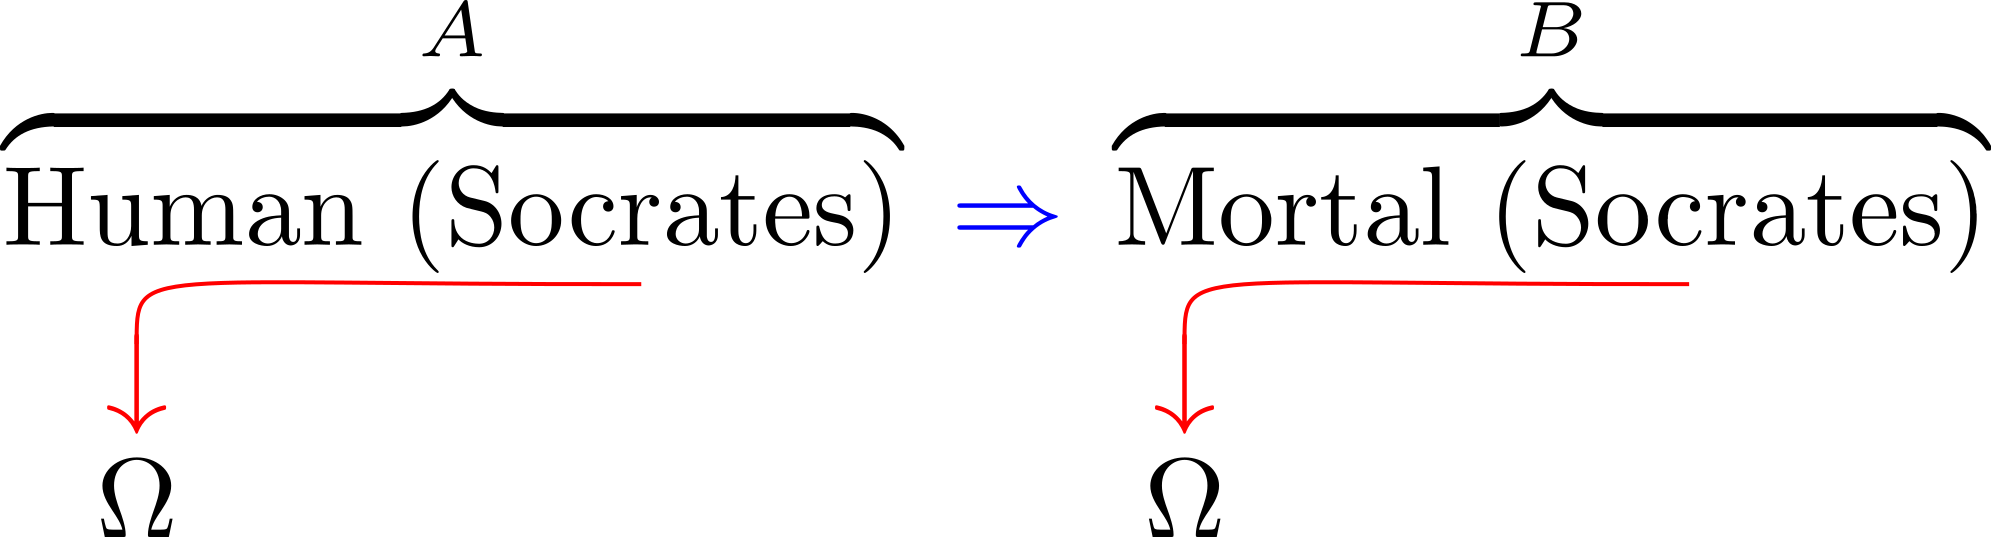
\includegraphics[scale=0.8]{why-Martin-Lof.png}}}
\end{equation}
{\color{red}红色 $\rightarrow$} 是 \textbf{predicates} 形成的层次。 $A$ 和 $B$ 是两个不同的\textbf{空间}。 在 $A$ \textbf{内部},Socrates 也是一个空间,Human 是另一个空间,而 Human(Socrates) 构成新的空间(透过 dependent type constructor $\Sigma$)。 

假设 $X \in \mathcal{U}_1, P \in \mathcal{U}_2, P(X) \in \mathcal{U}_3$,(这些 $\mathcal{U}_i$ 是 type universes), 在计算机上最简单的做法是令:
\begin{equation}
\mathcal{U}_3 = \mathcal{U}_1 \times \mathcal{U}_2
\end{equation}
这和 \S\ref{sec:Martin-Lof-TT} 说的 $\Sigma$ type constructor 本质上是 Cartesian product 的说法吻合。

到此,我们发现,用 Curry-Howard 的做法 和「粗暴」的 syntactic 做法其实是一模一样的! 有点失望,但我希望这些 漂亮的数学 不会是完全无用的....

\subsection{Implementation of topology (points and sets)}

是不是所有命题都 embed 到 命题空间 $\mathbb{P}\mathrm{rop}$?  还是有某种 working-space embedding?

这意思是说,从 long-term memory recall 进来,只要保证 inference makes sense 就行,constants 不必有长期的不变的位置。

或者可不可以说,是 constant 的 predicates 特性 决定其位置?

但 深度学习 似乎对 absolute positions 有优势。 例如「嫲嫲」的位置。 这是说,记忆中每个不同的客体 都有其 absolute position.  而另一种方法是 relative position: 从记忆中 recall 来的物体,附带 很多 predicates,但其 position 是 on-demand 建构的。 这两种做法有何分别? 似乎关键是 recall mechanism;

但回忆必需是一个带有 context 的整体。 问题是能不能做到 associative block recall.

这和 topology 有没有关? 可不可以用 LTM 减少 $F$ 的「负荷」? 换句话说 $F$ 只是负责 relative position 的 inference?  如果是 relative position 似乎有可能 reshape topology.  但仍是说不出 reshape topology 有什么好处,及其可能导致 errors 的问题.....

Reshape topology 带来 generalization 但也引入 errors.  

问题是如果用了 topology 那么 $F$ 会有哪些改变?  命题是 $P(a) = 1$.  它的信息 似乎无论如何也是一个 tuple $(P,a)$.  这会是一个 tuples to tuple 的 map,而这也就是 brutal syntactics.  但重点是: $P(a)$ 应该是一个\textbf{空间}。 这空间的构成是透过 type constructor $\displaystyle \sum_a P(a)$.  这构成一个空间,而 $F$ 是由 此空间到 彼空间 的一个映射。 於是 $F$ 并不是 tuples to tuple 的映射,而是 spaces to space 的映射。 
但这个映射是 witness 的映射,有点奇怪。 换句话说,要用 记忆体 记住 witnesses,它们代表每一个命题。 它们的位置就是命题的 syntax.  

在空间中有某个 witness, 它的位置 正是 $P(a)$ 的 positional tuple,它被映射到新位置也是 $Q(a)$ 的 positional tuple,这岂不是和 tuple to tuple 一模一样??  换句话说,无论怎样看,$F$ 的映射\textbf{必然是从 positional tuple to positional tuple}.

$P(a)$ 就是 $(P,a)$,syntactic mapping 是必然的。

那么 topology 又是什么?  $a$ 的位置是 $a$ 作为 Atom 的位置,它本身可以看成是一个 predicate.  但,个别的 constants 有没有永久的 位置?  如果位置是永久的,则 recall 非常容易(直接 recall)。 问题是要不要 reshape topology?  

另一个问题是: 开始时,一个 \textbf{新} constant 的位置是怎样 assign 的?  这显然和 \textbf{遗忘} 有关。  一个简单的做法就是有 \emp{constant 空间},而这些 constants \textbf{位置是永久的}。

所以又回到问题: 既然可以有 tuple-to-tuple, 那么 topological membership 要来做什么?  似乎就是用来 impose topological-metric \textbf{regularity} (ie, smoothness).

\subsection{Modal aspect}

\section{Model-based AI}

我提出的 BERT 的「逻辑化」AGI 模型 是基於 逻辑 syntax 的,换句话说是 用神经网络 模拟 $\vdash$,而这个 $\vdash$ 是 syntactic consequence.  现在考虑 $\models$,即 model-theoretic consequence.

最简单的 model 就是 point-set topology.  有如下对应:
\begin{eqnarray}
\mbox{propositions} & \Leftrightarrow & \mbox{points} \in \mbox{regions or product of domains} \\
\forall \mbox{ formulas} & \Leftrightarrow & \mbox{sub-regions} \nonumber
\end{eqnarray}

Model-based (logic-based) AI 的其中一个主要问题是: 在 syntax-based 情况下,我们可以在 working memory 引入一个命题 $P(a)$, 例如 $P =$「$a$ 是不是质数」,而可以暂时不理会 $P(x)$ 在其他点上的真值; 但在 model-based 情况下,model 包含了 $P$ 的 extension(= 一个点集 或 区域),这表示我们立即知道每一个数是不是质数,这是不切实际的。 这个问题或许可以称之为 ``\emp{omniscient predicates}'' 的问题。

Then what is inference?  What kind of changes would occur to the model?

Appearance of new propositions = appearance of new points / change of shape of regions.

\begin{equation}
\begin{tikzpicture}[overlay]
% \draw  plot[smooth, tension=.9] coordinates {(-2,0) (0,1) (2,0) (0,-1)  (-2,0)};
\draw (0,0) ellipse (3cm and 1cm);
\end{tikzpicture}
\bullet \mathrm{John}
\end{equation}

Then how is the spatial model better than a syntactic representation (bunch of propositions)?

\section*{References}
\cc{欢迎提问和讨论}{Questions, comments welcome} \smiley \\ \vspace*{0.4cm}
\printbibliography

\end{document} 
